\documentclass%
[handout]
{beamer}

% % % % % % % %
% % % % % % % %
% % % % % % % %
%IMPORTANT
%compiles with 
%pdflatex -shell-escape 
%IMPORTANT
% % % % % % % %
% % % % % % % %
% % % % % % % %


\usepackage{etex} %avoiding error: too many packages. This is a LaTeX bug (``feature'')


\mode<presentation>
{
\useinnertheme{rounded}
\useoutertheme{infolines}
\usecolortheme{orchid}
\usecolortheme{whale}
}

\usepackage[english]{babel}
\usepackage[latin1]{inputenc}
\usepackage[all,cmtip]{xy}
\usepackage{times}
\usepackage{auto-pst-pdf}
\usepackage{pstricks-add}
\usepackage{pst-plot}
\usepackage{pst-math}
\usepackage{pst-node}
\usepackage{cancel}

\usepackage[T1]{fontenc}
% Or whatever. Note that the encoding and the font should match. If T1
% does not look nice, try deleting the line with the fontenc.

\usepackage{../pstricks-commands}
\usepackage{../example-templates}
\graphicspath{{../../modules/}}

\setbeamertemplate{navigation symbols}{}

\includeonlylecture{4}

\newcommand{\lect}[3]{
  \date{#1}
  \lecture[#1]{#2}{#3}
}

\setbeamertemplate{footline}
{
  \leavevmode%
  \hbox{%
  \begin{beamercolorbox}[wd=.333333\paperwidth,ht=2.25ex,dp=1ex,center]{author in head/foot}%
    \usebeamerfont{author in head/foot}\insertshortauthor
  \end{beamercolorbox}%
  \begin{beamercolorbox}[wd=.333333\paperwidth,ht=2.25ex,dp=1ex,center]{title in head/foot}%
    \usebeamerfont{title in head/foot}\insertshorttitle
  \end{beamercolorbox}%
  \begin{beamercolorbox}[wd=.333333\paperwidth,ht=2.25ex,dp=1ex,center]{date in head/foot}%
    \usebeamerfont{date in head/foot}\insertshortdate{}
  \end{beamercolorbox}}%
  \vskip0pt%
}

% If you have a file called "university-logo-filename.xxx", where xxx
% is a graphic format that can be processed by latex or pdflatex,
% resp., then you can add a logo as follows:

%\pgfdeclareimage[height=0.8cm]{logo}{bluelogo}
%\logo{\pgfuseimage{logo}}

\begin{document}

\AtBeginLecture{%

\title[\insertlecture]{SFY0004}
\subtitle{\insertlecture}
\author[SFY0004]{Slides by Greg Maloney and Todor Milev}
\institute{Newcastle University}
\date{\insertshortlecture}
\begin{frame}
  \titlepage
\end{frame}

\begin{frame}{Outline}
  \tableofcontents[pausesections]
\end{frame}
}%

% begin lecture
\lect{January 31, 2014}{Lecture  2}{2}
\section{Module Information}
% begin module lecturer
\begin{frame}
\frametitle{Lecturer: Greg Maloney}
\begin{tabular}{rl}
office: & Herschel Building, 2.14 \\
email: & \texttt{gregory.maloney@ncl.ac.uk} \\
phone: & 01912087232 \\
consultation hours: & Th 13:30--14:30, F 10:30--11:30 \\
\end{tabular}
\end{frame}
% end module lecturer

% begin module homework
\begin{frame}
\frametitle{Homework}
\begin{itemize}
\item  There will be three homework assignments, worth a total of 10\% of the course grade.
\item  They will be due at the end of lecture on Friday of teaching weeks 2, 5, and 8.
\item  There are no extensions to homework deadlines.  Late homework will be examined and feedback given, but a mark of zero will be awarded.
\item  Each homework assignment will have a differentiation and an integration component.  
\item  The differentiation component will be distributed on Fridays.
\item  The integration component will be distributed on Mondays.
\end{itemize}
\end{frame}
% end module homework

\section{The Chain Rule}
% begin module chain-rule-intro-alternative
\begin{frame}
\frametitle{The Chain Rule}
\begin{itemize}
\item  What is the derivative of $F(x) = \cos x^3$?
\item<2->  The Power Rule doesn't tell us how to solve this.
\item<3->  $F$ is a composite function $f\circ g$:
\item<3-| alert@4-5,9,11-12>  $y = f(u) = \uncover<5->{\cos u}$.
\item<3-| alert@6-8,13-14>  $u = g(x) = \uncover<7->{x^3}$.
\item<3->  Then $y = F(x) = f(\alertNoH{ 8}{g(x)}) = \uncover<8->{\alertNoH{ 9}{f(\alertNoH{ 8}{x^3}) =}}  \uncover<9->{\alertNoH{ 9}{\cos x^3}.}$
\item<10->  We know the derivatives of $f$ and $g$:
\item<10-| alert@11-12>  $f'(u) = \uncover<12->{-\sin u}$.
\item<10-| alert@13-14>  $g'(x) = \uncover<14->{3x^2}$.
\item<15->  It would be nice if we could find the derivative of $F$ in terms of the derivatives of $y$ and $u$.
\item<16->  It turns out that the derivative of the composition $f\circ g$ is the product of the derivative of $f$ and the derivative of $g$.
\item<17->  This important fact is called the Chain Rule.
\end{itemize}
\end{frame}
% end module chain-rule-intro-alternative

% begin module chain-rule-statement
\begin{frame}
The Chain Rule

If $g$ is differentiable at $x$ and $f$ is differentiable at $g(x)$, then the composite function $F = f\circ g$ defined by $F(x) = f(g(x))$ is differentiable at $x$ and $F'$ is given by the product
\[
F'(x) = f'(g(x))\cdot g'(x)
\]
In Leibniz notation, if $y = f(u)$ and $u = g(x)$ are both differentiable functions, then
\[
\frac{\diff y}{\diff x} = \frac{\diff y}{\diff u} \frac{\diff u}{\diff x}
\]

\uncover<2->{%
We will not prove this in class, but a proof can be found on p. 204 of the textbook.
}%
\end{frame}
% end module chain-rule-statement

% begin module chain-rule-cos-poly.tex
\begin{frame}
\chainruley{\cos x^3}{x^3}{\cos u}{-\sin UU}{3x^2}{-3x^2 \sin UU}{0}
\end{frame}
% end module chain-rule-cos-poly.tex
% begin module chain-rule-poly-cos.tex
\begin{frame}
\chainruley{\cos^3 x}{\cos x}{u^3}{3 UU^2}{-\sin x}{-3\sin x (UU)^2}{0}
\end{frame}
% end module chain-rule-poly-cos.tex
% begin module chain-rule-power-rule
\begin{frame}
\begin{itemize}
\item  In the example $y = \sin^2 x$, the outer function was a power function: $y = u^2$.
\item<2->  The derivative was $\frac{\diff y}{\diff x} = 2u \frac{\diff u}{\diff x} = 2\sin x \cos x$.
\item<3->  We can generalize this:
\end{itemize}

\uncover<3->{%
The Power Rule Combined with the Chain Rule

If $n$ is any real number and $u = g(x)$ is differentiable, then
\[
\frac{\diff}{\diff x} (u^n) = nu^{n-1} \frac{\diff u}{\diff x}
\]
Alternatively,
\[
\frac{\diff}{\diff x}[g(x)]^n = n [g(x)]^{n-1} \cdot g'(x)
\]
}%
\end{frame}
% end module chain-rule-power-rule

% begin module chain-rule-ex3
\begin{frame}
\[
\frac{\diff}{\diff x}(u^n) = nu^{n-1}\frac{\diff u}{\diff x}
\]
\chainruley{(x^3-1)^{100}}{x^3-1}{u^{100}}{100UU^{99}}{3x^2}{300x^2(UU)^{99}}{Example 3, p. 159}
\end{frame}
% end module chain-rule-ex3

% begin module chain-rule-ex4
\begin{frame}
\[
\frac{\diff}{\diff x}[g(x)]^n = n[g(x)]^{n-1}\cdot g'(x)
\]
\chainrulefofx{\frac{1}{\sqrt[3]{x^2+x+1}}}{x^2+x+1}{x^{-1/3}}{-\frac{1}{3}(UU)^{-4/3}}{2x+1}{-\frac{2x+1}{3}(UU)^{-4/3}}{}
\end{frame}
% end module chain-rule-ex4

% begin module chain-rule-ex5
\begin{frame}
\begin{example}[Example 5, p. 201]
Find the derivative of
\[
g(t) = \left( \frac{t-2}{2t+1}\right)^9.
\]
\abovedisplayskip=0pt
\belowdisplayskip=0pt
\abovedisplayshortskip=0pt
\belowdisplayshortskip=0pt
\begin{align*}
&  \uncover<2->{\text{Power Rule and Chain Rule:}}\\%
\uncover<2->{%
g'(t)%
}%
& \uncover<2->{ = } %
\uncover<2->{%
9\left( \frac{t-2}{2t+1}\right)^8 \alert<handout:0| 3-4>{\frac{\diff}{\diff t}\left( \frac{t-2}{2t+1}\right)}%
}\\%
&  \uncover<3->{\text{Quotient Rule:}}\\%
& \uncover<3->{ = } %
\uncover<3->{%
9\left( \frac{t-2}{2t+1}\right)^8 \alert<handout:0| 3-4>{\frac{(2t+1)\alert<handout:0| 5-6>{\frac{\diff}{\diff t}(t-2)}-(t-2)\alert<handout:0| 7-8>{\frac{\diff}{\diff t}(2t+1)}}{(2t+1)^2}}%
}\\%
& \uncover<5->{ = } %
\uncover<5->{%
9\left( \frac{t-2}{2t+1}\right)^8 \frac{(2t+1)\cdot \alert<handout:0| 5-6>{\uncover<6->{1}}-(t-2)\cdot \alert<handout:0| 7-8>{\uncover<8->{2}}}{(2t+1)^2}%
}\\%
& \uncover<9->{ = } %
\uncover<9->{%
9\left( \frac{t-2}{2t+1}\right)^8 \frac{2t+1-2t+4}{(2t+1)^2}%
}  \uncover<10->{ = } \uncover<10->{%
\frac{45(t-2)^8}{(2t+1)^{10}}%
}%
\end{align*}
\end{example}
\end{frame}
% end module chain-rule-ex5

% begin module chain-rule-extra-links
\begin{frame}
\begin{itemize}
\item  We can add more ``links'' when we use the Chain Rule.
\item<2-| alert@3>  $y = f(u)$
\item<2-| alert@4>  $u = g(x)$
\item<2-| alert@4>  $x = h(t)$
\item<3->  Use the Chain Rule twice:
\end{itemize}
\[
\uncover<3->{%
\alert<handout:0| 3>{\frac{\diff y}{\diff t} = \frac{\diff y}{\diff u}\alert<handout:0| 4>{\frac{\diff u}{\diff t}}}%
}%
\uncover<4->{%
 = \frac{\diff y}{\diff u}\alert<handout:0| 4>{\frac{\diff u}{\diff x}\frac{\diff x}{\diff t}}%
}%
\]
\end{frame}
% end module chain-rule-extra-links

% begin module chain-rule-twice-ex3
\begin{frame}
\chainruletwice%
{\tan \Big( \frac{1}{x^2+1}\Big)}%
{\sec^2 \Big( \frac{1}{x^2+1}\Big)}%
{\frac{1}{x^2+1}}%
{\frac{-1}{(x^2+1)^2}}%
{x^2+1}%
{2x}%
{}%
{-\frac{2x\sec^2 \Big( \frac{1}{x^2+1}\Big)}{(x^2+1)^2}}%
{}%
\end{frame}
% end module chain-rule-twice-ex3

% end lecture

% begin lecture
\lect{February 7, 2014}{Lecture  4}{4}
\section{Exponential Functions}
\subsection{Definition and Properties}
% begin module exponential-function-def
\begin{frame}
\frametitle{ %(1.2) 
Exponential Functions}
The function $f(x) = 2^x$ is called an exponential function because the variable $x$ is the exponent.
\begin{columns}[c]
\column{.5\textwidth}
\psset{xunit=0.8cm, yunit=0.8cm}
\begin{pspicture}(-2.5,-0.5)(2.5,6.25)
\psframe*[linecolor=white](-2.5,-0.5)(2.5,6.25)
\psaxes[labels=none]{<->}(0,0)(-2.5,-0.5)(2.5,6.25)
\rput[t](1, -0.2){$1$}
\uncover<3->{
\psFullDot{2}{4}
}
\uncover<5->{
\psFullDot{1}{2}
}
\uncover<7->{
\psFullDot{0}{1}
}
\uncover<9->{
\psFullDot{-1}{0.5}
}
\uncover<11->{
\psFullDot{-2}{0.25}
}
\uncover<12->{
\rput[r](-0.5, 1.5){$y=2^x$}
%Function formula: 2^{x} 
\psplot[linecolor=red, plotpoints=1000]{-2.5}{2.5}{2 x exp }
}
\end{pspicture}
%\only<handout:0| -2>{%
%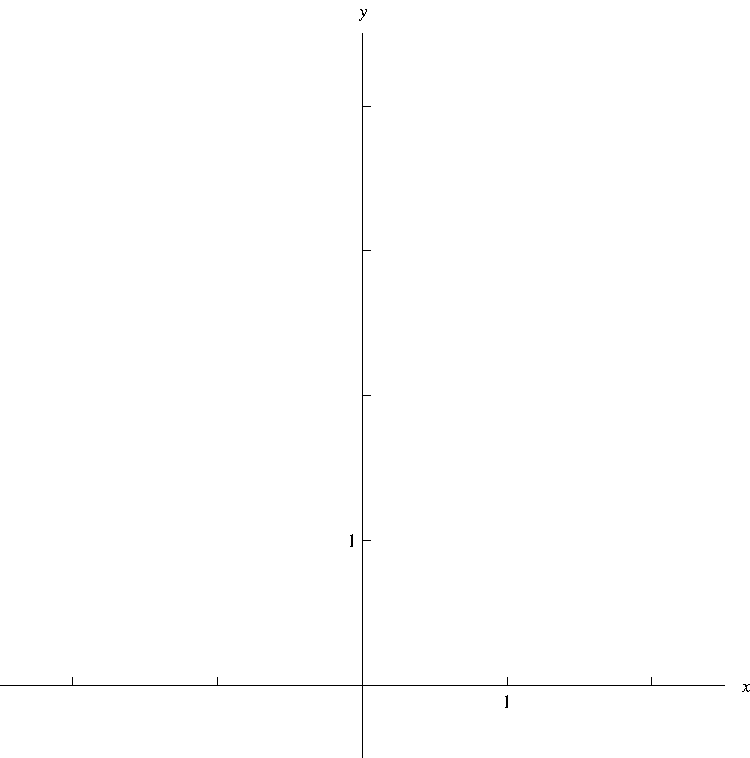
\includegraphics[height=6cm]{exponential-functions/pictures/twoxa.pdf}%
%}%
%\only<handout:0| 3-4>{%
%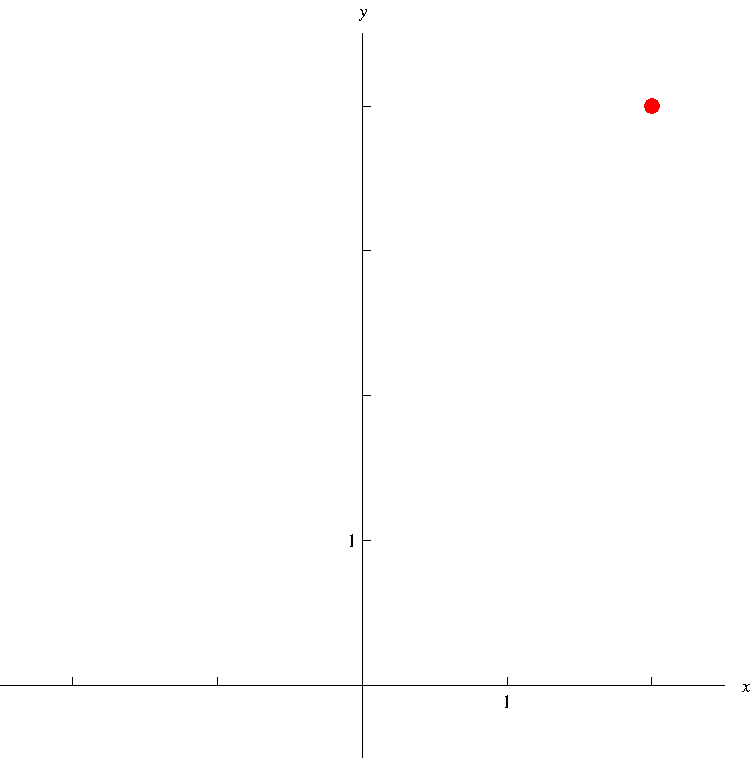
\includegraphics[height=6cm]{exponential-functions/pictures/twoxb.pdf}%
%}%
%\only<handout:0| 5-6>{%
%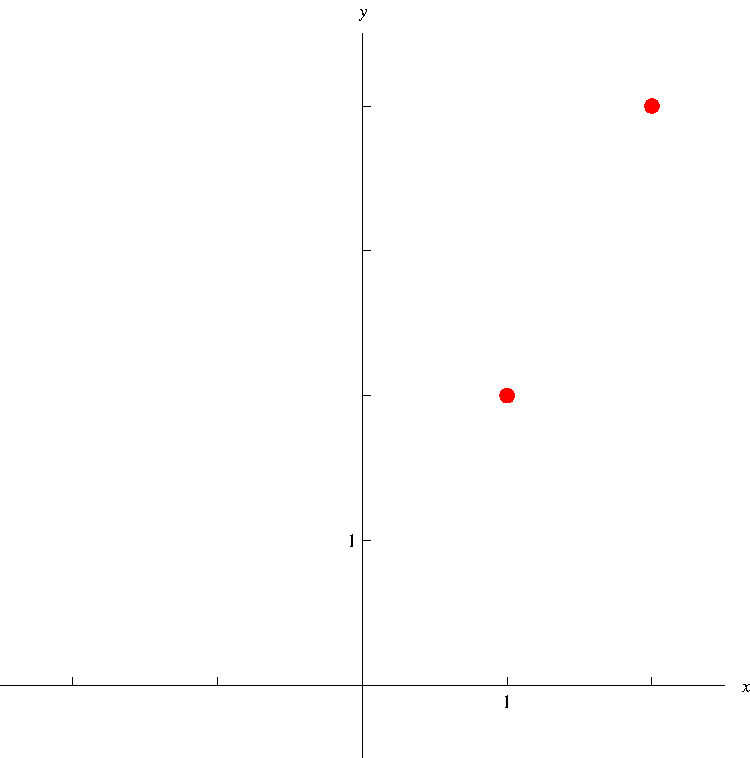
\includegraphics[height=6cm]{exponential-functions/pictures/twoxc.pdf}%
%}%
%\only<handout:0| 7-8>{%
%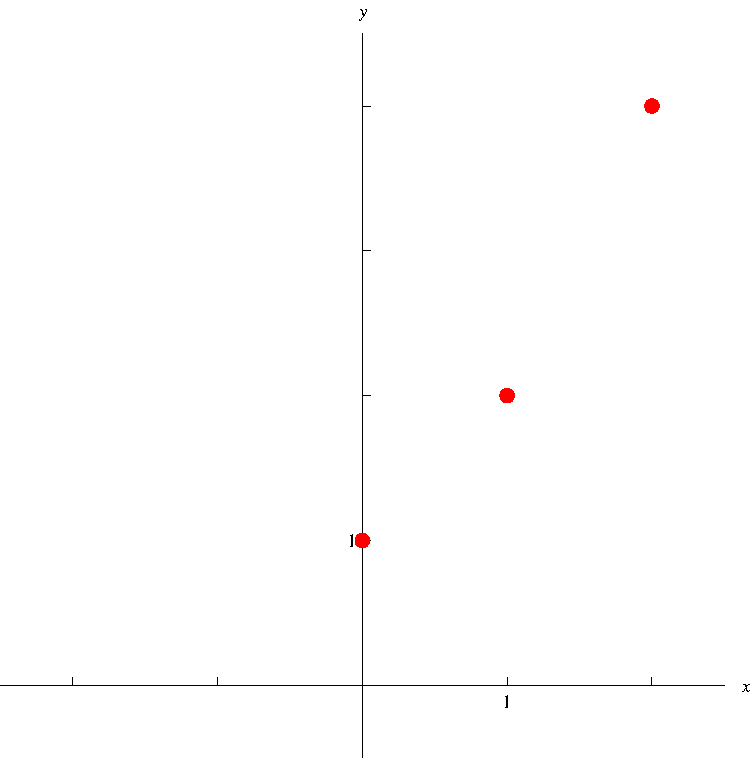
\includegraphics[height=6cm]{exponential-functions/pictures/twoxd.pdf}%
%}%
%\only<handout:0| 9-10>{%
%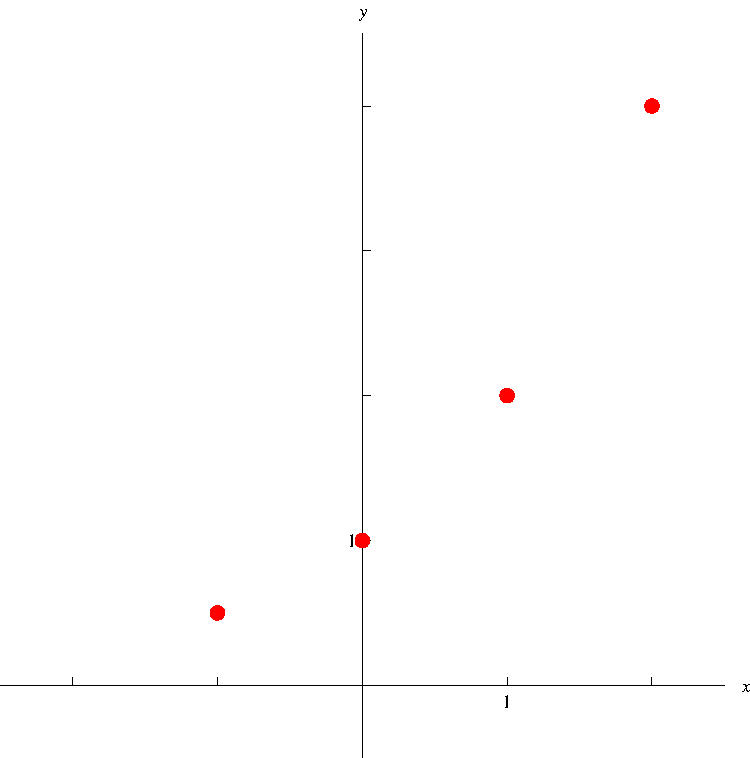
\includegraphics[height=6cm]{exponential-functions/pictures/twoxe.pdf}%
%}%
%\only<handout:0| 11>{%
%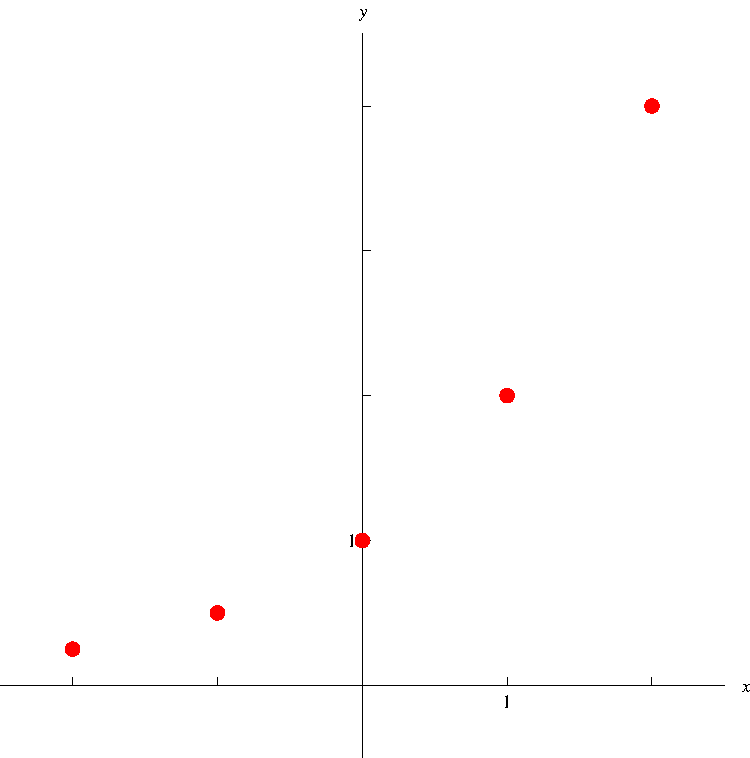
\includegraphics[height=6cm]{exponential-functions/pictures/twoxf.pdf}%
%}%
%\only<handout:1| 12->{%
%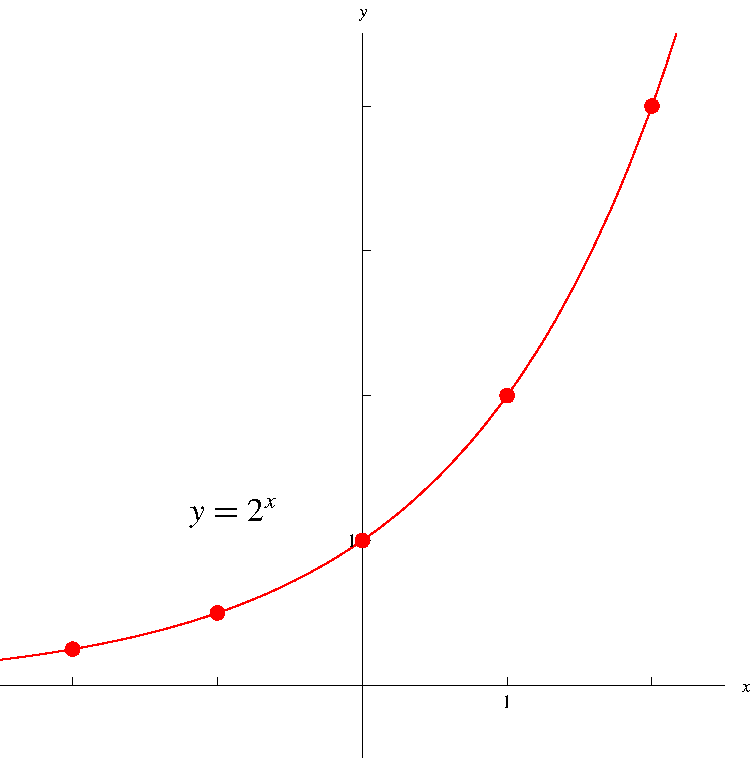
\includegraphics[height=6cm]{exponential-functions/pictures/twoxg.pdf}%
%}%


\column{.5\textwidth}
\[
\begin{array}{r|l}
x & y\\
\hline
\alert<handout:0| 2-3>{2} & \alert<handout:0| 3>{\uncover<3->{4}} \\
\alert<handout:0| 4-5>{1} & \alert<handout:0| 5>{\uncover<5->{2}} \\
\alert<handout:0| 6-7>{0} & \alert<handout:0| 7>{\uncover<7->{1}} \\
\alert<handout:0| 8-9>{-1} & \alert<handout:0| 9>{\uncover<9->{1/2}} \\
\alert<handout:0| 10-11>{-2} & \alert<handout:0| 11>{\uncover<11->{1/4}} 
\end{array}
\]
\uncover<13->{
\begin{definition}[Exponential Function]
An exponential function is a function of the form $f(x) = a^x$, where $a$ is a positive constant.
\end{definition}
}
\end{columns}
\end{frame}
% end module exponential-function-def
% begin module exponential-function-graphs-plus
\begin{frame}
\begin{columns}
\column{0.7\textwidth}
Graphs of various exponential functions.

\psset{xunit=2cm, yunit=2cm}
\begin{pspicture}(-2.1,-0.2)(2.2,3.6) 
\psframe*[linecolor=white](-2.1,-0.2)(2.1,3.5)
\psaxes[labels=none]{<->}(0,0)(-2.1,-0.2)(2.1,3.5)
\uncover<1->{
\rput[r](1.8, 2.3){$y=2^x$}
%Function formula: 2^{x} 
\psplot[linecolor=red, plotpoints=1000]{-2}{1.584962501}{2 x exp }
}
\uncover<2->{
\rput[l](0.7, 3.1){$y=4^x$}
%Function formula: 4^{x} 
\psplot[linecolor=black, plotpoints=1000]{-2}{0.79248125}{4 x exp }
}
\uncover<3->{
\rput[b](0.4, 3.05){$y=10^x$}
%Function formula: 4^{x} 
\psplot[linecolor=blue, plotpoints=1000]{-2}{0.477121255}{10 x exp }
}
\uncover<4->{
\rput[l](1.15, 1.5){$y=1.5^x$}
%Function formula: 4^{x} 
\psplot[linecolor=green, plotpoints=1000]{-2}{2}{1.5 x exp }
}
\uncover<5->{
\rput[l](-1.9, 2){$y=0.5^x$}
%Function formula: 4^{x} 
\psplot[linecolor=purple, plotpoints=1000]{-1.584962501}{2}{0.5 x exp }
}
\uncover<6->{
\rput[l](-1.2, 3.1){$y=0.25^x$}
%Function formula: 4^{x} 
\psplot[linecolor=brown, plotpoints=1000]{-0.79248125}{2}{0.25 x exp }
}
\end{pspicture}

\column{0.3\textwidth}
\uncover<7->{Observations}
 
\begin{itemize}
\item<8-| alert@8-9> $a^x$ is always \uncover<9->{positive.}  
\item<10-| alert@10-11> $a^0 = \uncover<11->{1}$ for all $a$.  
\end{itemize}
\uncover<12->{$a > 1$:}
\begin{itemize}
\item<12-| alert@12-13> $\displaystyle \lim_{x\to\infty}a^x = \uncover<13->{\infty.}$
\item<12-| alert@14-15> $\displaystyle \lim_{x\to-\infty}a^x = \uncover<15->{0.}$
\end{itemize}
\uncover<12->{$a < 1$:}
\begin{itemize}
\item<12-| alert@16-17> $\displaystyle \lim_{x\to\infty}a^x = \uncover<17->{0.}$
\item<12-| alert@18-19> $\displaystyle \lim_{x\to-\infty}a^x = \uncover<19->{\infty.}$
\end{itemize}
\end{columns}

\end{frame}
% end module exponential-function-graphs-plus

% begin module exponential-properties
\begin{frame}[t]
Properties of exponential expressions.  

\uncover<8->{Suppose $a$ is positive.  Then}
\begin{enumerate}
\item<8->  $a^xa^y = a^{x+y}$
\item<15->  $\frac{a^x}{a^y} = a^{x-y}$
\item<20->  $(a^x)^y = a^{xy}$
\item<28->  $(ab)^x = a^xb^x$
\end{enumerate}

\only<-8| handout:0>{%
\begin{align*}
\uncover<2->{\alert<2-3>{2^3}\cdot \alert<4-5>{2^2} & = \alert<2-3>{(\uncover<3->{2\cdot 2\cdot 2})}\alert<4-5>{(\uncover<5->{2\cdot 2})} } \\
\uncover<6->{ & = 2\cdot 2\cdot 2\cdot 2\cdot 2 } \\
\uncover<7->{ & = 2^5.}
\end{align*}
}%

\only<9-15| handout:0>{%
\begin{align*}
\uncover<9->{\frac{\alert<9-10>{2^3}}{\alert<11-12>{2^2}} & = \frac{\alert<9-10>{\uncover<10->{\alert<13>{2\cdot 2}\cdot 2}}}{\alert<11-13>{\uncover<12->{2\cdot 2}}} } \\
\uncover<13->{ & = 2 } \\
\uncover<14->{ & = 2^1.}
\end{align*}
}%

\only<16-20| handout:0>{%
\begin{align*}
\uncover<16->{(2^2)^4 & = 2^2\cdot 2^2\cdot2^2\cdot 2^2 } \\
\uncover<17->{ & = (2\cdot 2)(2\cdot 2)(2\cdot 2)(2\cdot 2) } \\
\uncover<18->{ & = 2\cdot2\cdot2\cdot2\cdot2\cdot2\cdot2\cdot2 } \\
\uncover<19->{ & = 2^8 } 
\end{align*}
}%

\only<21-28| handout:0>{%
\begin{align*}
\uncover<21->{(2\cdot 3)^3 & = (2\cdot 3)(2\cdot 3)(2\cdot 3) } \\
\uncover<22->{ & = 2\cdot 3 \cdot 2\cdot 3 \cdot 2\cdot 3 } \\
\uncover<23->{ & = \alert<24-25>{2\cdot 2 \cdot 2}\cdot \alert<26-27>{3 \cdot 3\cdot 3} } \\
\uncover<24->{ & = \alert<24-25>{\uncover<25->{2^3}} \cdot \alert<26-27>{\uncover<27->{3^3}} } 
\end{align*}
}%

\end{frame}
% end module exponential-properties

% begin module exponential-equation1
\begin{frame}
\begin{example}[Solving an exponential equation]
Solve for $t$.  
\begin{align*}
16^{4t} & = 8^{t-2} \\
\uncover<2->{\text{Find a common base:}\quad \alert<2-3>{\big( \uncover<3->{2^4}\big)}^{4t}} & \uncover<2->{ = \alert<2-3>{\big( \uncover<3->{2^3}\big)}^{t-2} } \\
\uncover<4->{2^{16t}} & \uncover<4->{ = 2^{3t-6}} \\
\uncover<5->{16t} & \uncover<5->{ = 3t - 6} \\
\uncover<6->{13t} & \uncover<6->{ =  -6} \\
\uncover<7->{t} & \uncover<7->{ =  -6/13.} 
\end{align*}
\end{example}
\end{frame}
% end module exponential-equation1

% begin module exponential-word-problem1
\begin{frame}
\begin{example}[Solving an exponential word problem]
A farmer buys \alert<handout:0| 8>{$48$ chickens} and \alert<handout:0| 10>{$6$ rabbits}.
\alert<handout:0| 8>{The chicken population doubles each year}, and \alert<handout:0| 10>{the rabbit population doubles every six months.}
\alert<handout:0| 3>{When} does the farmer have \alert<handout:0| 5>{the same} \alert<handout:0| 4,6>{number of} \alert<handout:0| 4>{chickens} as \alert<handout:0| 6>{rabbits}?

\uncover<2->{%
Let $c(t)$ denote the number of chickens after $t$ years, and let $r(t)$ denote the number of rabbits after $t$ years.
}%
\abovedisplayskip=0pt
\belowdisplayskip=0pt
\begin{align*}
\uncover<3->{\alert<3| handout:0>{\text{Solve for $t$:}}}\quad  \uncover<4-| handout:0>{\alertNoH{4,7-8}{c(t)}} & \uncover<5->{\alert<5| handout:0>{=}} \uncover<6-| handout:0>{\alertNoH{6,9-10}{r(t)}} \\
\uncover<8-| handout:0>{\alertNoH{8}{\alertNoH{11}{48}\cdot 2^t}} & \uncover<7->{=} \uncover<10-| handout:0>{\alertNoH{10}{\alertNoH{11}{6}\cdot 4^t}} \\
\uncover<11-| handout:0>{\alertNoH{11-13}{8}\cdot 2^t} & \uncover<11->{=} \uncover<11-| handout:0>{\alertNoH{14-15}{4^t}} \\
\uncover<12-| handout:0>{\text{Find a common base:}\quad \alertNoH{12-13}{2^{\uncover<13->{3}}}\cdot 2^t } & \uncover<12->{=} \uncover<12-| handout:0>{\alertNoH{14-15}{2^{\uncover<15->{2t}}}} \\
\uncover<16-| handout:0>{2^{t+3}} & \uncover<16->{=} \uncover<16-| handout:0>{2^{2t}} \\
\uncover<17-| handout:0>{t+3} & \uncover<17->{=} \uncover<17-| handout:0>{2t} \\
\uncover<18->{t} & \uncover<18->{=} \uncover<18-| handout:0>{3.}
\end{align*}
\uncover<19-| handout:0>{Therefore the chicken and rabbit populations are equal after $3$ years.}
\end{example}
\end{frame}
% end module exponential-word-problem1

% begin module exponential-equation2
\begin{frame}
\begin{example}[Solving a quadratic exponential equation]
Solve for $x$.  
\abovedisplayskip=0pt
\belowdisplayskip=0pt
\begin{align*}
9^x & = 2\cdot 3^x + 63 \\
\uncover<2-| handout:0>{\alert<handout:0| 4-5>{9^x} -2\cdot \alert<handout:0| 3>{3^x} - 63} & \uncover<2->{ = 0} \\
\intertext{\uncover<3->{Substitute $\alert<handout:0| 9>{u = \uncover<3-| handout:0>{3^x}}$:}}
\uncover<3-| handout:0>{\alert<handout:0| 4-5>{\uncover<5->{u^2}} - 2\alert<handout:0| 3>{u} - 63} & \uncover<3->{ = 0} \\
\uncover<6->{\alert<handout:0| 6-7>{(\uncover<7-| handout:0>{u-9})(\uncover<7-| handout:0>{u+7})}} & \uncover<6->{ = 0 } 
\end{align*}
\begin{align*}
\uncover<8->{ \alert<handout:0| 9>{u} } & \uncover<8->{ = \uncover<8-| handout:0>{9} } & \uncover<8->{\text{or}} & & \uncover<8->{\alert<handout:0| 9>{u}} & \uncover<8->{ = \uncover<8-| handout:0>{-7}} \\
\uncover<9-| handout:0>{ \alert<handout:0| 9>{3^x} } & \uncover<9-| handout:0>{ = 9 } & \uncover<9-| handout:0>{\text{or}} & & \uncover<9-| handout:0>{\alert<handout:0| 9>{3^x}} & \uncover<9-| handout:0>{ = -7} \invisible{99999999} \\
\uncover<10-| handout:0>{ \alert<handout:0| 10-11>{x} } & \uncover<10-| handout:0>{ \alert<handout:0| 10-11>{ = \uncover<11->{2} }} & & & \uncover<10-| handout:0>{\alert<handout:0| 12-13>{\uncover<-12>{x}}} & \uncover<10-| handout:0>{ \alert<handout:0| 12-13>{ \only<-12>{ =} \only<13->{\text{no solution}} }} 
\end{align*}
\uncover<14-| handout:0>{Therefore $x = 2$ is the solution.}
\end{example}
\end{frame}
% end module exponential-equation2

% end lecture

% begin lecture
\lect{February 14, 2014}{Lecture  6}{6}
\section{Exponential Functions}
\subsection{The Natural Exponential Function}
% begin module exponential-function-derivative
\begin{frame}
\frametitle{Derivatives of Exponential Functions}
Compute the derivative of $f(x) = a^x$ using the definition:
\begin{align*}
\uncover<2->{f'(x) = \lim_{h\to 0} \frac{f(x+h)-f(x)}{h}} & \uncover<3->{=}  \uncover<3->{\lim_{h\to 0} \frac{\alert<handout:0| 4>{a^{x+h}}-a^x}{h}}\\
 & \uncover<4->{=}  \uncover<4->{\lim_{h\to 0} \frac{\alert<handout:0| 5>{\alert<handout:0| 4>{a^x a^h}-a^x}}{h}}\\
 & \uncover<5->{=}  \uncover<5->{\lim_{h\to 0} \frac{\alert<handout:0| 5>{\alert<handout:0| 6>{a^x} (a^h- 1)}}{h}}\\
 & \uncover<6->{=}  \uncover<6->{\alert<handout:0| 6>{a^x} \alert<handout:0| 7>{\lim_{h\to 0} \frac{a^h- 1}{h}}}\\
 & \uncover<7->{=}  \uncover<7->{a^x \alert<handout:0| 7>{f'(0)}.}
\end{align*}
\end{frame}


\begin{frame}
We have shown that, if $f(x) = a^x$ is differentiable at 0, then it is differentiable everywhere, and
\[
f'(x) = f'(0)a^x .
\]
\uncover<2->{
We leave the following theorem without proof. 
\begin{theorem}
Let $a$ be a positive number and let $f(x)=a^x$. Then the limit \[f'(0)=\lim_{h\rightarrow 0}\frac{a^h - 1}{h}\] exists. 
\end{theorem}

In fact, it can be shown, as was/will be done in Calculus I that the limit above equals $\ln a$, i.e., $f'(0)=\ln(a)$. Here, $\ln$ is the natural logarithm function (was/will be defined in Calculus I).
}
\end{frame}
% end module exponential-function-derivative

% begin module e-def
\begin{frame}
\[
\text{If}\quad  f(x) = a^x, \quad \text{then}\quad f'(x) = f'(0)a^x .
\]
The simplest differential formula occurs when $f'(0) = 1$.  Since $\lim_{h\rightarrow 0}\frac{2^h-1}{h}\approx 0.69$ and $\lim_{h\rightarrow 0}\frac{3^h-1}{h}\approx 1.10$, we expect there is a number $a$ between 2 and 3 such that $\lim_{h\rightarrow 0}\frac{a^h-1}{h} = 1$.  
\uncover<2->{
\begin{definition}[$e$]
$e$ is the number such that $\lim_{h\rightarrow 0}\frac{e^h-1}{h} = 1$.
\end{definition}
}

\begin{columns}
\column{.3\textwidth}
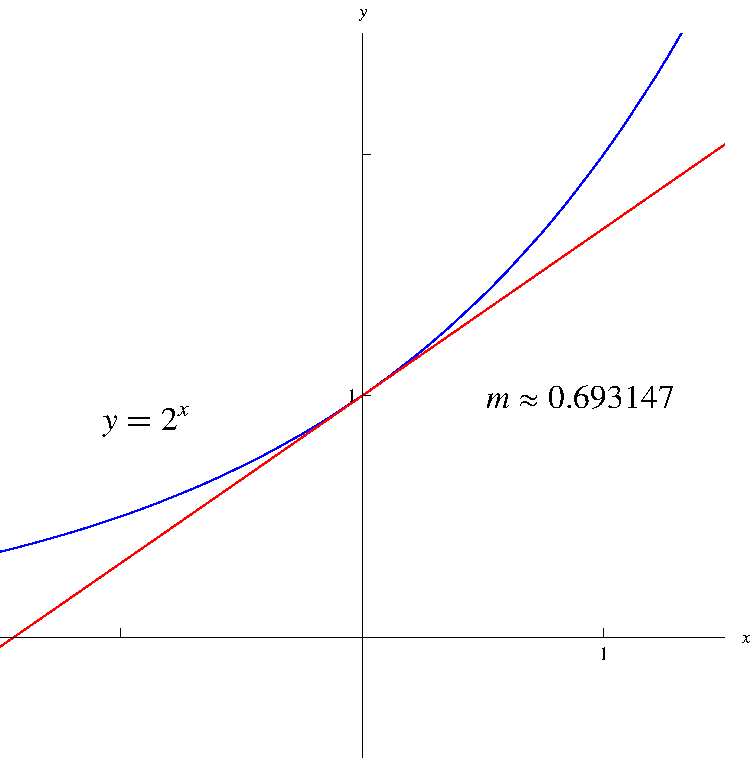
\includegraphics[height=4cm]{exponential-functions/pictures/exp-tangent-two.pdf}%
\column{.3\textwidth}
\uncover<handout: 1|3->{%
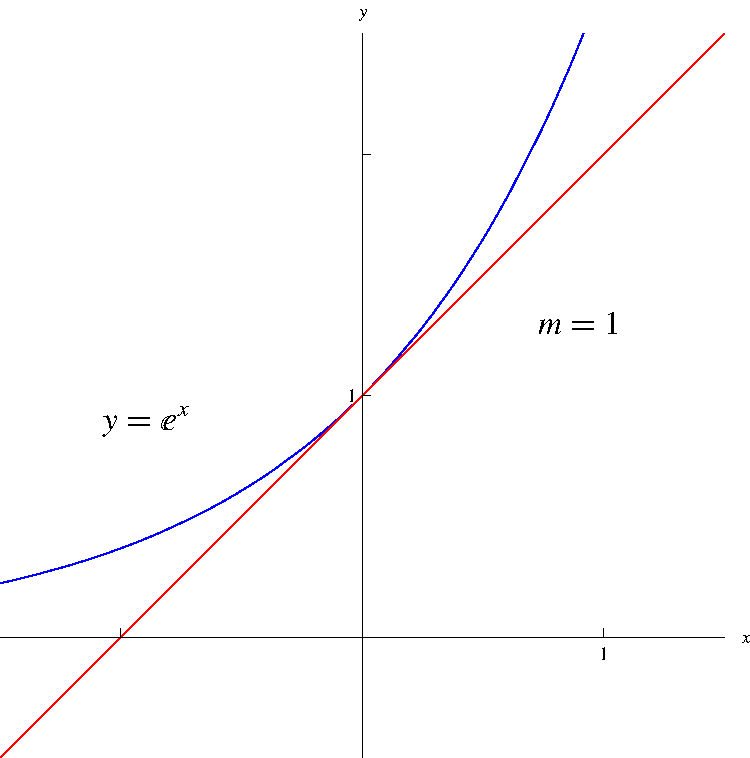
\includegraphics[height=4cm]{exponential-functions/pictures/exp-tangent-e.pdf}%
}%
\column{.3\textwidth}
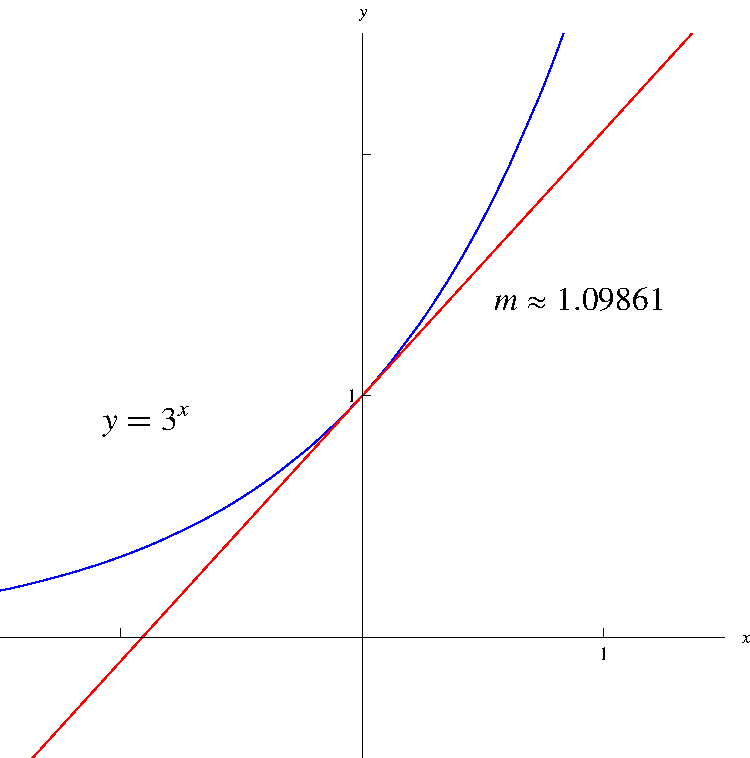
\includegraphics[height=4cm]{exponential-functions/pictures/exp-tangent-three.pdf}%
\end{columns}
\end{frame}
% end module e-def

% begin module natural-exponential-def
\begin{frame}
\begin{definition}[Natural Exponential Function]
$e^x$ is called the natural exponential function.  Its derivative is
\[
\frac{\diff}{\diff x} e^x = e^x .
\]
\end{definition}
\uncover<2->{
We can use this fact to find an approximation for $e$:
}
\begin{itemize}
\item<3->  Let $\alert<handout:0| 7,12>{e = 2^c}$.
\item<4->  Let $f(x) = 2^x$.  Then $\alert<handout:0| 8>{f'(x) = k2^x}$, where $\alert<handout:0| 13>{k = f'(0) \approx 0.693147}$.
\item<5->  $\alert<handout:0| 6>{e^x = \uncover<6->{\frac{\diff}{\diff x} (\alert<handout:0| 7>{e^x})}} \uncover<7->{ = \alert<handout:0| 8>{\frac{\diff}{\diff x} (\alert<handout:0| 7>{2^{cx}})}} \uncover<8->{\alert<handout:0| 8>{= k2^{cx}\frac{\diff}{\diff x} (cx) }} \uncover<9->{= ck 2^{cx}.}$
\item<10->  Substitute $x = 0$: $1 = e^0 = ck2^0 = ck$.
\item<11->  Therefore $\alert<handout:0| 12>{c = 1/k}$.
\item<12->  $\alert<handout:0| 12>{e = 2^{1/\alert<handout:0| 13>{k}}} \uncover<13->{ \approx 2^{1/\alert<handout:0| 13>{0.693147}}} \uncover<14->{\approx 2.71828 .}$
\end{itemize}
\end{frame}
% end module natural-exponential-def

% begin module derivative-e-plus-polynomial
\begin{frame}
\begin{example}[Derivative of a Polynomial and the Natural Exponential Function]
\abovedisplayskip=0pt
\belowdisplayskip=-15pt
\abovedisplayshortskip=0pt
\belowdisplayshortskip=0pt
\begin{align*}
\text{Differentiate}\quad y & = e^x+x^7.\\
\uncover<2->{\frac{\diff y}{\diff x} & = \frac{\diff}{\diff y}(\alert<3-4>{e^x}) + \frac{\diff}{\diff y}(\alert<5-6>{x^7})}\\
& \uncover<3->{= \uncover<4->{\alert<4>{e^x}}  + \uncover<6->{\alert<6>{7x^6}.}}
\end{align*}
\end{example}
\end{frame}
% end module derivative-e-plus-polynomial
% begin module chain-rule-e
\begin{frame}
\chainruley{e^{-3x}}{-3x}{e^{u}}{e^{UU}}{-3}{-3e^{UU}}{Natural Exponential Function}
\end{frame}
% end module chain-rule-e

% begin module chain-rule-twice-ex2
\begin{frame}
\chainruletwice%
{ e^{\tan \left(\pi x\right)}}%
{e^{\tan \left(\pi x\right)}}%
{\tan\left(\pi x\right)}%
{\sec^2 \left(\pi x\right)}%
{\pi x}%
{\pi}%
{}%
{\pi e^{\tan \left(\pi x\right)}\sec^2 \left(\pi x\right)}%
{}%
\end{frame}
% end module chain-rule-twice-ex2

\section{Inverse Functions}
\subsection{One-to-one Functions}
% begin module one-to-one-def
\begin{frame}
\frametitle{One-to-one Functions}
\begin{definition}[One-to-one Function]
A function $f$ is a one-to-one function if it never takes on the same value twice; that is,
\[
f(x_1) \neq f(x_2) \ \text{whenever }  \ x_1 \neq x_2 .
\]
\end{definition}
\begin{columns}[c]
\column{.5\textwidth}
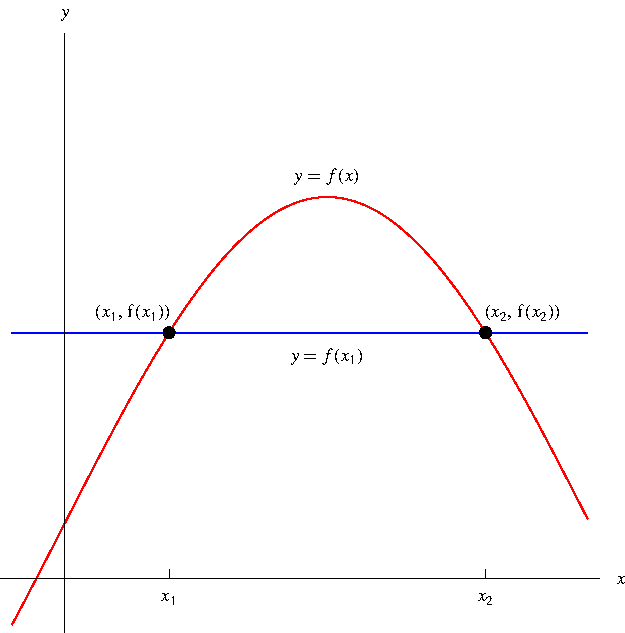
\includegraphics[height=5cm]{inverse-functions/pictures/07-01-1-1def.pdf}%
\column{.5\textwidth}
$\leftarrow$ This function is not one-to-one.
\end{columns}
\end{frame}
% end module one-to-one-def

% begin module horizontal-line-test
\begin{frame}
Question: How can we tell from the graph of a function whether it is one-to-one or not?

Answer: Use the horizontal line test.

\begin{proof}[The Horizontal Line Test]
A function is one-to-one if and only if no horizontal line intersects it more than once.
\end{proof}

\begin{tabular}{cc}
\psset{xunit=0.7cm, yunit=0.7cm}
\begin{pspicture}(-5, -5)(5,5) 
\psframe*[linecolor=white](-5,-5)(5,5) 
\psaxes[ticks=none, labels=none]{<->}(0,0)(-3,-3)(3,3)
%Function formula: 1/2 (x)+1/2 
\psplot[linecolor=red, plotpoints=1000]{1}{2}{0.5 x 0.5 mul add } %Function formula: (x)^{3} 
\psplot[linecolor=red, plotpoints=1000]{-1}{1}{x 3 exp } %Function formula: 3/2 (x)+1/2 
\psplot[linecolor=red, plotpoints=1000]{-2}{-1}{0.5 x 1.5 mul add }
\end{pspicture} 
%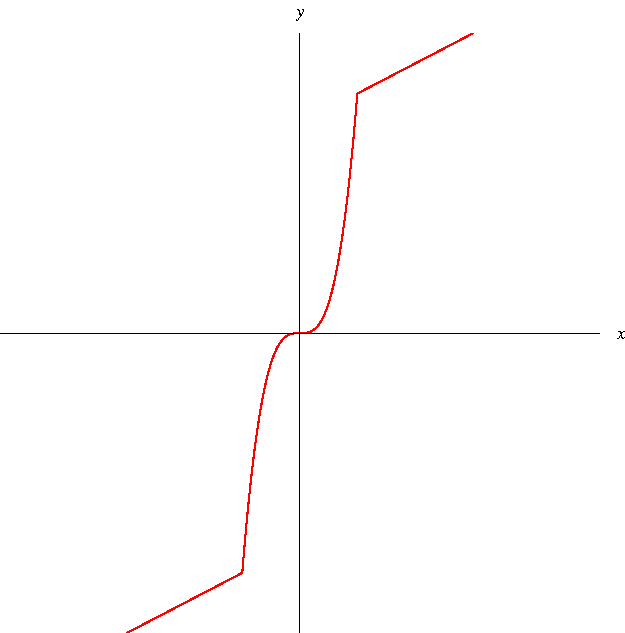
\includegraphics[height=4cm]{inverse-functions/pictures/07-01-onetoone.pdf} 
 %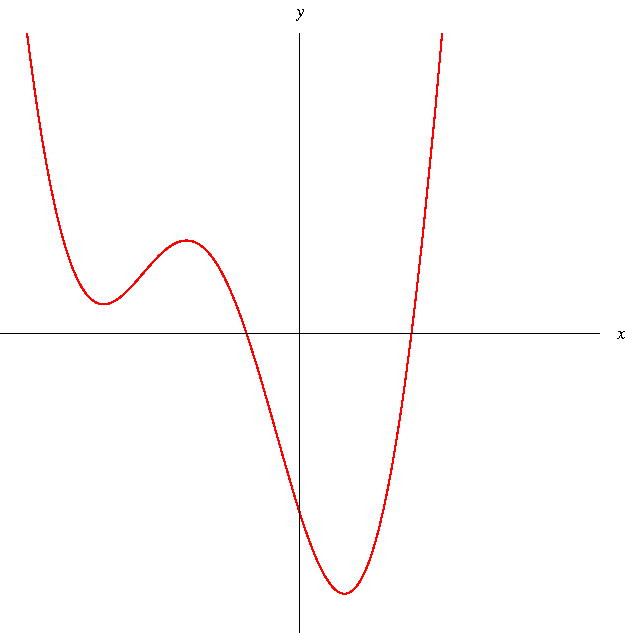
\includegraphics[height=4cm]{inverse-functions/pictures/07-01-notonetoonea.pdf}%
&%
\uncover<handout:0| 2->{%
\psset{xunit=0.7cm, yunit=0.7cm}
\begin{pspicture}(-5, -5)(5,5) 
\psframe*[linecolor=white](-5,-5)(5,5) 
\psaxes[ticks=none, labels=none]{<->}(0,0)(-3,-3)(3,3)
 %Function formula: -2/5+((6/5+x)^{2}) ((x) (x))-6/25 ((6/5+x)^{2})- (((6/5+x)^{2}) (x)) 
 \psplot[linecolor=red, plotpoints=1000]{-2}{1.5}{x x 1.2 add 2 exp mul -1 mul x 1.2 add 2 exp -0.24 mul add x x mul x 1.2 add 2 exp mul add -0.4 add }
 \uncover<3->{
 \psline[linestyle=dashed](-3, 1)(3, 1)
 }
 \end{pspicture} 
}
\\
\uncover<2->{\alert<handout:0| 2>{One-to-one}} &
\uncover<3->{\alert<handout:0| 3>{Not one-to-one}}
\end{tabular}
\end{frame}
% end module horizontal-line-test

\subsection{The Definition of the Inverse of $f$}
% begin module inverse-function-def
\begin{frame}
\frametitle{The Definition of the Inverse of $f$}
\begin{definition}[$f^{-1}$]
Let $f$ be a one-to-one function with domain $A$ and range $B$.  Then the inverse of $f$ is the function $f^{-1}$ that has domain $B$ and range $A$ and is defined by
\[
f^{-1}(y) = x \qquad \Leftrightarrow \qquad f(x) = y 
\]
for all $y$ in $B$.
\end{definition}
\begin{columns}[T]
\column{.5\textwidth}
\uncover<2->{Note:}
\begin{itemize}
\item<3->  Only one-to-one functions have inverses.
\item<4->  $f^{-1}$ reverses the effect of $f$.
\item<5->  domain of $f^{-1} = $ range of $f$.
\item<5->  range of $f^{-1} = $ domain of $f$.
\end{itemize}
\column{.5\textwidth}
\uncover<6->{
\begin{example}[$f(x) = x^3$]
The inverse of $f(x) = x^3$ is $f^{-1}(x) = \sqrt[3]{x}$.  This is because if $y = x^3$, then
\[
f^{-1}(y) = \sqrt[3]{y} = \sqrt[3]{x^3} = x .
\]
\end{example}
}
\end{columns}
\end{frame}
% end module inverse-function-def

% begin module inverse-notation-warning
\begin{frame}
\alert<1->{WARNING:}

Do not mistake the $-1$ in $f^{-1}(x)$ for an exponent.
\[
f^{-1}(x) \ \text{does not mean } \ \frac{1}{f(x)} .
\]

If you want to write $\frac{1}{f(x)}$ using exponents, you can write $(f(x))^{-1}$.
\begin{itemize}
\item<2->  $f^{-1}(x)$ is the compositional inverse of $f$.
\item<3->  $\frac{1}{f(x)}$ is the multiplicative inverse of $f$.
\end{itemize}
\end{frame}
% end module inverse-notation-warning

% begin module inverse-function-solve-for
\begin{frame}
\frametitle{How to Find the Inverse of a One-to-one Function}
\begin{enumerate}
\item<1-| alert@3>  Write $y = f(x)$.
\item<1-| alert@4-5>  Solve this equation for $x$ in terms of $y$ (if possible).
\item<1-| alert@6>  Interchange $x$ and $y$.  The resulting equation is $y = f^{-1}(x)$. 
\end{enumerate}
\uncover<2->{
\begin{example}%[Example 4, p. 388]
If $f(x) = x^3 + 2$, find a formula for $f^{-1}(x)$.
\begin{align*}
\uncover<3->{y} & \uncover<3->{=}  \uncover<3->{x^3 + 2}\\
\uncover<4->{x^3} & \uncover<4->{=}  \uncover<4->{y - 2}\\
\uncover<5->{\alert<handout:0| 6>{x}} & \uncover<5->{=}  \uncover<5->{\sqrt[3]{\alert<handout:0| 6>{y} - 2}}\\% 
\uncover<6->{\alert<handout:0| 6>{y}} & \uncover<6->{=}  \uncover<6->{\sqrt[3]{\alert<handout:0| 6>{x} - 2}} \qquad \uncover<6->{\alert<handout:0| 6>{\text{(New equation.)}}}
\end{align*}
\uncover<7->{
Therefore $f^{-1}(x) = \sqrt[3]{x - 2}$.
}
\end{example}
}
\end{frame}
% end module inverse-function-solve-for

% begin module guess-and-check
\begin{frame}
\begin{example}[Guess and Check]
If $f(x) = 2x + \sin 2x + e^{x/2}$, find $f^{-1}(1)$.  
\begin{align*}
\uncover<2->{f\alert<handout:0| 2-3>{(\uncover<3->{0})}} & \uncover<2->{=}  \uncover<2->{2\alert<handout:0| 2-3>{(\uncover<3->{0})}  + \sin 2\alert<handout:0| 2-3>{(\uncover<3->{0})}  + e^{\alert<handout:0| 2-3>{(\uncover<3->{0})}/2} }\\ 
 & \uncover<2->{=}  \uncover<3->{0 + 0 + 1} \\
 & \uncover<2->{=}  \uncover<2->{1.} \\
\uncover<4->{\text{Therefore}\quad f^{-1}(1)} & \uncover<4->{=}  \uncover<4->{0.}
\end{align*}
\end{example}
\end{frame}
% end module guess-and-check

% begin module inverse-function-graph
\begin{frame}
\begin{tabular}{cc}
\psset{xunit=1cm, yunit=1cm}
\begin{pspicture}(-5, -5)(5,5) 
\psframe*[linecolor=white](-5,-5)(5,5) 
\psaxes[ticks=none, labels=none]{<->}(0,0)(-1.5,-1.5)(3.4,3.1)
\psLabels{3.4}{3.1}
\uncover<6->{
\psline(2.5, 1)(1, 2.5)
\psline(1.85, 1.65)(1.95, 1.75)(1.85, 1.85)
\psline(1.85, 1.85)(1.75, 1.95)(1.65, 1.85)

\psline(1.9875, 1.3125)(2.1875, 1.5125)
\psline(2.0625, 1.2375)(2.2625, 1.4375)
\psline(1.3125, 1.9875)(1.5125, 2.1875)
\psline(1.2375, 2.0625)(1.4375, 2.2625)

\psline[linecolor=blue](-1.35, -1.35)(2.8,2.8)
\rput[l](-1, -1.2){\footnotesize $y=x$}
}
\uncover<2->{
\psFullDot{2.5}{1}
\rput[lt](2.6, 1.1){\footnotesize $(a,b)$}
}
\uncover<5->{
\psFullDot{1}{2.5}
\rput[rb](0.9, 2.6){\footnotesize $(b,a)$}
}
\end{pspicture}
%\ \only<handout:0| -4>{%
%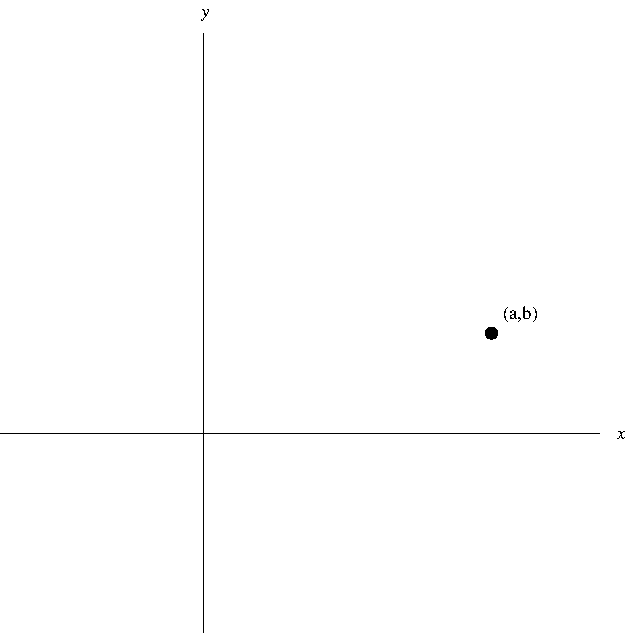
\includegraphics[height=4cm]{inverse-functions/pictures/07-01-reflecta.pdf}%
%}%
%\only<handout:0| 5>{%
%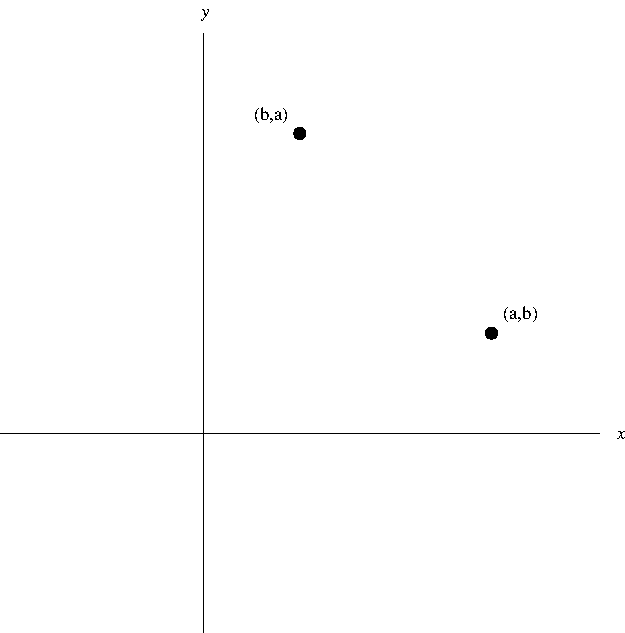
\includegraphics[height=4cm]{inverse-functions/pictures/07-01-reflectb.pdf}%
%}%
%\only<handout:1| 6->{%
%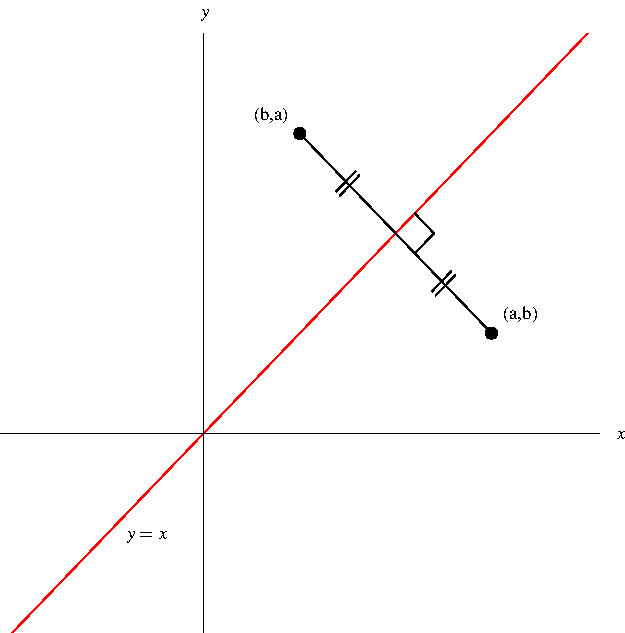
\includegraphics[height=4cm]{inverse-functions/pictures/07-01-reflectc.pdf}%
%}%
&%
\psset{xunit=1cm, yunit=1cm}
\begin{pspicture}(-5, -5)(5,5) 
\psframe*[linecolor=white](-5,-5)(5,5) 
\psaxes[ticks=none, labels=none]{<->}(0,0)(-1.55,-1.5)(3.4,3.1)
\psLabels{3.4}{3.1}
\uncover<7->{
\psline(0.75, 2.36359)(2.36359, 0.75)
\psline(1.65679, 1.65679)(1.55679, 1.75679)(1.45679, 1.65)
\psline(1.65679, 1.65679)(1.75679, 1.55679)(1.65679, 1.45679)
\psFullDot{0.75}{2.36359}
\psFullDot{2.36359}{0.75}

\psline[linecolor=blue](-1.35, -1.35)(2.8,2.8)
\rput[l](-1, -1.2){\footnotesize $y=x$}
\psplot[linecolor=red, plotpoints=1000]{-0.292893219}{3}{x 1 add ln  0.693147181 div 1 sub}
\rput[lb](0.9, 2.4){\footnotesize $y=f^{-1}(x)$}
%Function formula: 2^{1+x}-1 
\psplot[linecolor=red, plotpoints=1000]{-1.5}{0.95}{-1 2 x 1 add exp add }
\psline[linecolor=blue](-1.4, -1.4)(2.9,2.9)
\rput[l](-1, -1.2){\footnotesize $y=x$}
\rput[tr](2.8, 0.4){\footnotesize $y=f(x)$}
}
\end{pspicture} 
%\only<handout:0| -6>{%
%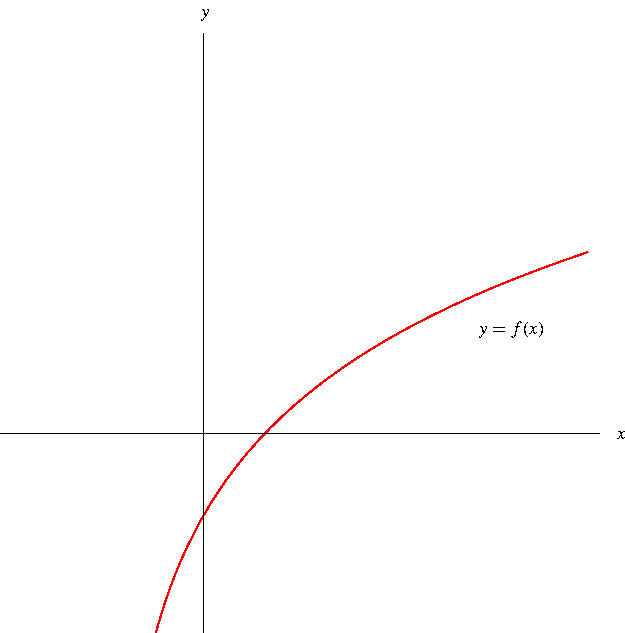
\includegraphics[height=4cm]{inverse-functions/pictures/07-01-reflect-functionb.pdf}%
%}%
%\only<handout:1| 7->{%
%\includegraphics[height=4cm]{inverse-functions/pictures/07-01-reflect-f unctiona.pdf}%
%}%
\end{tabular}

\footnotesize 
Interchanging $x$ and $y$ suggests a relation between the graphs of $f^{-1}$ and $f$:
\begin{itemize}
\item<2->  Suppose $(a,b)$ is on the graph of $f$.
\item<3->  Then $f(a) = b$.
\item<4->  Then $f^{-1}(b) = a$.
\item<5->  Then $(b,a)$ is on the graph of $f^{-1}$.
\item<6->  $(b,a)$ is the reflection of $(a,b)$ in the line $y = x$.
\item<7->  Therefore the graph of $f^{-1}$ is obtained by reflecting the graph of $f$ across the line $y = x$.
\end{itemize}
\end{frame}
% end module inverse-function-graph

% begin module inverse-function-ex5
\begin{frame}
\begin{example}%[Example 5, p. 388]
\begin{columns}[c]
\column{.5\textwidth}
\psset{xunit=0.5cm, yunit=0.5cm}
\begin{pspicture}(-5, -5)(5,5) 
\psframe*[linecolor=white](-5,-5)(5,5) \tiny
\psaxes[ticks=none, labels=none]{<->}(0,0)(-4.55,-5)(4.5,5)
\psline(1, -0.1)(1, 0.1)
\rput[t](1, -0.2){\tiny$1$}
\psline(-1, -0.1)(-1, 0.1)
\psline(-0.1, 1)(0.1, 1)
\rput[br](-0.2, 1){\tiny$1$}
\psline(-0.1, -1)(0.1, -1)
\uncover<3>{
%Function formula: sqrt{}(- (x)) 
\psplot[linecolor=red, plotpoints=1000]{-4.5}{0}{x -1 mul sqrt }
\rput(-2, 2.2){\tiny$y=\sqrt{-x}$}
}
\uncover<4->{
%Function formula: sqrt{}(- (x)) 
\psplot[linecolor=gray, plotpoints=1000]{-4.5}{0}{x -1 mul sqrt }
\rput(-2, 2.2){\color{gray}\tiny$y=\sqrt{-x}$}
}
\uncover<2>{
 %Function formula: sqrt{}(x) 
\psplot[linecolor=red, plotpoints=1000]{0}{4.5}{x sqrt } 
\rput(2.4, 1){\tiny $y=\sqrt{x}$}
}
\uncover<3->{
 %Function formula: sqrt{}(x) 
\psplot[linecolor=gray, plotpoints=1000]{0}{4.5}{x sqrt } 
\rput(2.4, 1){\color{gray}\tiny $y=\sqrt{x}$}
}
\uncover<4>{
%Function formula: sqrt{}(- (x)-1) 
\psplot[linecolor=red, plotpoints=1000]{-4.5}{-1}{-1 x -1 mul add sqrt }
\rput[r](-2.3, 0.55){\tiny$y=f(x)$}
}
\uncover<5->{
%Function formula: sqrt{}(- (x)-1) 
\psplot[linecolor=gray, plotpoints=1000]{-4.5}{-1}{-1 x -1 mul add sqrt }
\rput[r](-2.3, 0.55){\color{gray}\tiny$y=f(x)$}
}

\uncover<5>{
%Function formula: - ((x)^{2})-1 
\psplot[linecolor=red, plotpoints=1000]{0}{2}{-1 x 2 exp -1 mul add } 
\rput[l](1.3, -2){\tiny$y=f^{-1}(x)$}
\psline[linecolor=blue, linestyle=dashed] (-4.5, -4.5)(4.5, 4.5)
\rput[tl](-3, -3.2){\tiny $y=x$}
}
\end{pspicture} 
%\ \only<handout:0| -1>{%
%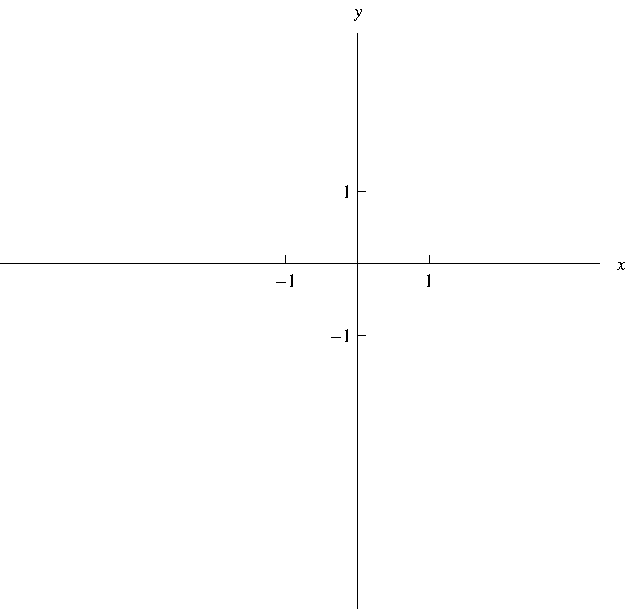
\includegraphics[height=4.5cm]{inverse-functions/pictures/07-01-ex5a.pdf}%
%}%
%\only<handout:0| 2>{%
%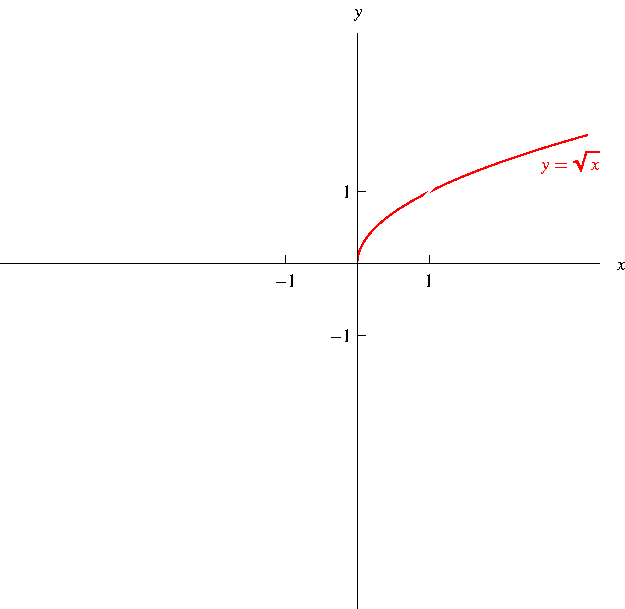
\includegraphics[height=4.5cm]{inverse-functions/pictures/07-01-ex5b.pdf}%
%}%
%\only<handout:0| 3>{%
%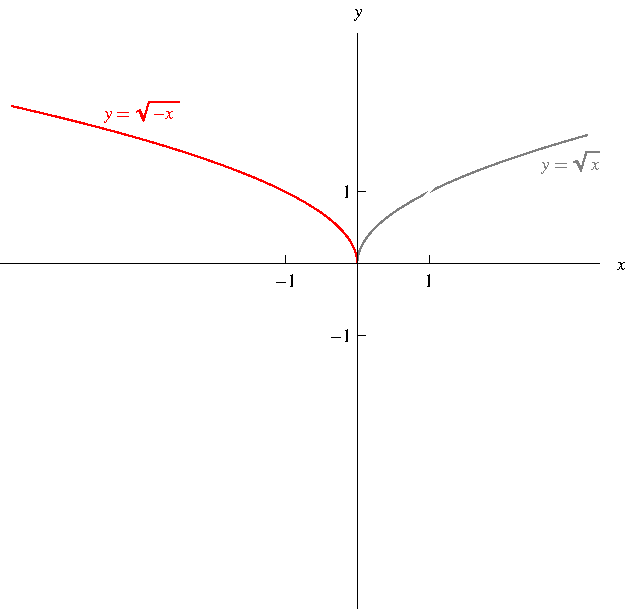
\includegraphics[height=4.5cm]{inverse-functions/pictures/07-01-ex5c.pdf}%
%}%
%\only<handout:0| 4>{%
%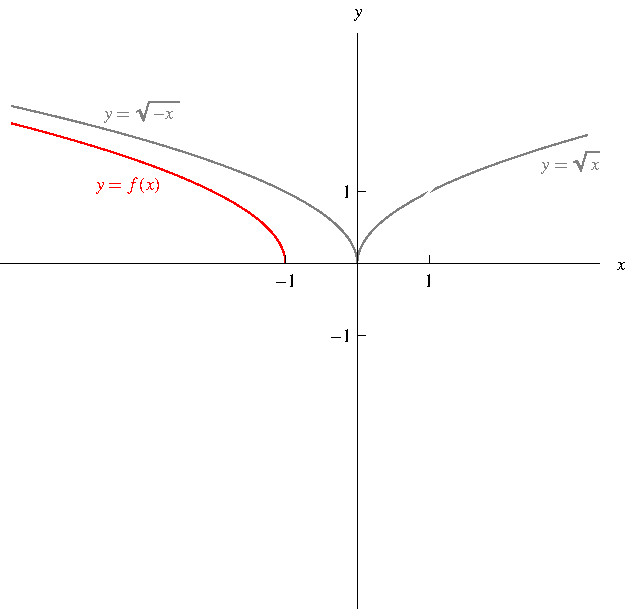
\includegraphics[height=4.5cm]{inverse-functions/pictures/07-01-ex5d.pdf}%
%}%
%\only<handout:1| 5->{%
%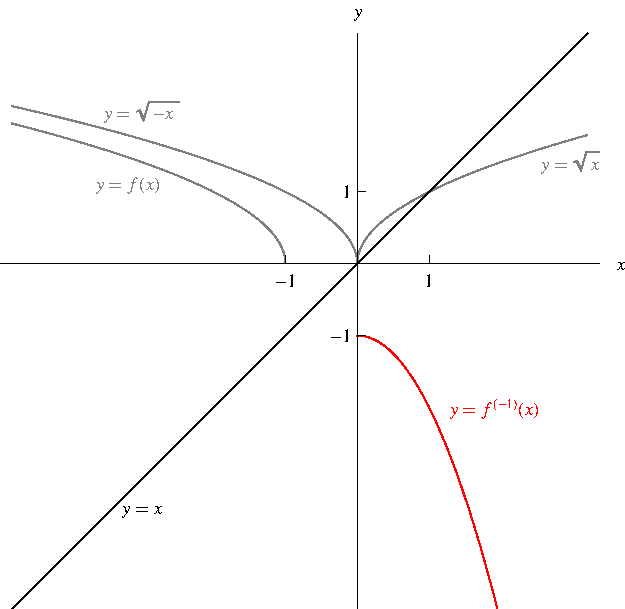
\includegraphics[height=4.5cm]{inverse-functions/pictures/07-01-ex5e.pdf}%
%}%

\column{.5\textwidth}
Sketch the graph of $f(x) = \sqrt{-x - 1}$ and its inverse function.
\end{columns}
\begin{itemize}
\item<2->  First draw the graph of $y = \sqrt{x}$.
\item<3->  $y = \sqrt{-x}$ is the reflection of $y = \sqrt{x}$ in the $y$-axis.
\item<4->  $y = f(x) = \sqrt{-x - 1}$ is the shift of $y = \sqrt{-x}$ one unit to the left.
\item<5->  $y = f^{-1}(x)$ is the reflection of $y = f(x)$ across the line $y = x$.
\end{itemize}
\end{example}
\end{frame}
% end module inverse-function-ex5
% begin module inverse-function-solve-for
\begin{frame}
%\frametitle{Inverse of a ne-to-one Function}
\begin{example}[\uncover<16->{\alert<handout:0| 16,17>{What if we change the problem to $x\leq -\frac{2}3$?}}]
Given: $\alert<handout:0| 2>{f(x) =  3x^2+4x-7}$ \alert<handout:0| 3,16,17>{with domain $x\only<1-16| handout:0>{\geq}\only<17->{\leq} -\frac{2}{3}$}.  Find $f^{-1}(x)$.
\begin{columns}
\column{0.4\textwidth}
\psset{xunit=0.35cm, yunit=0.35cm}
\begin{pspicture}(-9,-9)(5,5)
\psframe*[linecolor=white](-9,-9)(5,5)
\tiny
\psaxes[ticks=none, labels=none]{<->}(0,0)(-9,-9)(4.7,4.7)
\uncover<2-16| handout:0>{ %
\psplot[linecolor=\fcColorGraph, plotpoints=1000] {-0.66}{1.401612274}{x 2 exp 3 mul x 4 mul add -7 add }
}
\uncover<17->{ %
\psplot[linestyle=dashed, linecolor=gray!50, plotpoints=1000]{-0.66}{1.401612274}{x 2 exp 3 mul x 4 mul add -7 add }
}
\uncover<2,17>{ %
\psplot[linecolor=\fcColorGraph, plotpoints=1000]{-2.7349}{-0.67}{x 2 exp 3 mul x 4 mul add -7 add }
}
\uncover<3-16| handout:0>{ %
\psplot[linestyle=dashed, linecolor=gray!50, plotpoints=1000] {-2.7349}{-0.67}{x 2 exp 3 mul x 4 mul add -7 add }
}
\uncover<14->{
\psline[linecolor=blue, linestyle=dashed](-6.5, -6.5)(4.5,4.5)
}
\uncover<15-16| handout:0>{
\psplot[linecolor=red, plotpoints=1000]{-8.33333}{4.5}{-0.666667 25 x 3 mul add sqrt 0.333333 mul add }
}
\uncover<17->{
\psplot[linestyle=dashed, linecolor=gray!50, plotpoints=1000] {-8.33333}{4.5}{-0.666667 25 x 3 mul add sqrt 0.333333 mul add }
}
\uncover<15-16>{
\psplot[linecolor=gray!50, linestyle=dashed, plotpoints=1000] {-8.33333}{4.5}{-0.666667 25 x 3 mul add sqrt -0.333333 mul add }
}
\uncover<17->{
\psplot[linecolor=\fcColorGraph, plotpoints=1000] {-8.33333}{4.5}{-0.666667 25 x 3 mul add sqrt -0.333333 mul add }
}
\uncover<15-16| handout:0>{\rput[lb](-6, 1){$y=f^{-1}(x)$}}
\uncover<11->{\rput (-3.5, -8 ){$(-\frac{2}{3}, -\frac{25}{3})$}}
\uncover<2-16| handout:0>{\rput[tl](1.8, 4.45){$y=f(x)$}}
\uncover<14->{\rput[l] (-7.8, -2.2 ){$(-\frac{25}{3}, -\frac{2}{3})$}}
\uncover<17->{\rput[rt](4.5, -3){$y=f^{-1}(x)$}}
\uncover<17>{ \rput[tr](-3, 4.5){$y=f(x)$}}
\uncover<14->{\fcFullDot{-8.33333}{-0.666667}}
\fcFullDot{-0.666667}{-8.33333}
\end{pspicture}
\uncover<13->{Final }\uncover<12->{answer}\uncover<13->{, \alert<handout:0| 13>{relabelled}:}
\[
\uncover<12->{
f^{-1}(\only<12| handout:0>{y}\only<13->{\alert<handout:0| 13>{x}} )=-\frac{2}{3} \only<1-16| handout:0>{+}\only<17->{\alert<handout:0| 17>{-}} \frac{\sqrt{25 +3\only<12| handout:0>{y} \only<13->{\alert<handout:0| 13>{x}}\phantom{y} }}{3}\quad.
}
\]

\column{0.6\textwidth}

\[\begin{array}{rcl}
\uncover<4->{3x^2+4x-7&=&y } \\
\uncover<4->{\alert<handout:0| 7>{3}x^2+\alert<handout:0| 6>{4}x+\alert<handout:0| 8>{(-7-y)}&=&0 }
\end{array}
\]
\uncover<5->{That's \alert<handout:0| 6,7,8>{a quadratic equation in $x$}. Solve:}
\[\begin{array}{l}
\uncover<5->{
\phantom{=}\displaystyle \frac{-\alert<handout:0| 6>{4} \pm \sqrt{\alert<handout:0| 6>{4}^2-4\cdot\alert<handout:0| 7>{3}\cdot\alert<handout:0| 8>{(-y-7)} }}{2\cdot\alert<handout:0| 7>{3}} \\
%~&=& \frac{-2 \pm \sqrt{25+3y}}{3}\\
}
\\
\uncover<9->{=\displaystyle-\frac{2 \pm \sqrt{25+3y}}{3}=} \uncover<10->{\displaystyle-\frac{2}3 \pm \frac{\sqrt{25+3y}}{3}\quad .}
\end{array}
\]
\uncover<11->{
We are given $x\only<11-16| handout:0>{\geq}\only<17->{\alert<handout:0| 17>{\leq}}-\frac{2}3 $, therefore $x=-\frac{2}{3}\only<11-16| handout:0>{+}\only<17->{\alert<handout:0| 17>{-}}\frac{\sqrt{25+3y}}{3}=f^{-1}(y)$.
}
\end{columns}
\vspace{-10pt}
\end{example}
\end{frame}
% end module inverse-function-solve-for

% end lecture

% begin lecture
\lect{February 21, 2014}{Lecture  8}{8}
\section{Logarithmic Functions}
\subsection{Definition and Properties}
% begin module logarithm-def
\begin{frame}
\frametitle{Logarithmic Functions}
\begin{columns}[c]
\column{.3\textwidth}
\psset{xunit=0.7cm, yunit=0.7cm}
\begin{pspicture}(-2,-2.1)(4.2, 4.2)
\psframe*[linecolor=white](-2,-2.1)(4.2, 4.2)
\psaxes[ticks=none, labels=none]{<->}(0,0)(-2,-2.1)(4.2, 4.2)
\psline(-0.1, 1)(0.1,1)
\rput[r](-0.2, 1){\footnotesize$1$}
\rput(0.9, 3){\footnotesize$y=a^x$}
%Function formula: 2^{x} 
\psplot[linecolor=red, plotpoints=1000]{-2}{2}{2 x exp }
\uncover<8->{
\psplot[linecolor=red, plotpoints=1000]{0.25}{4}{x ln 0.693147181 div }
\psline[linestyle=dashed, linecolor=blue](-1.9, -1.9)(4,4) 
\rput[tl](2, 0.7){\footnotesize$y=\log_ax$}
}
\end{pspicture} 
%\ \only<handout:0| -7>{%
%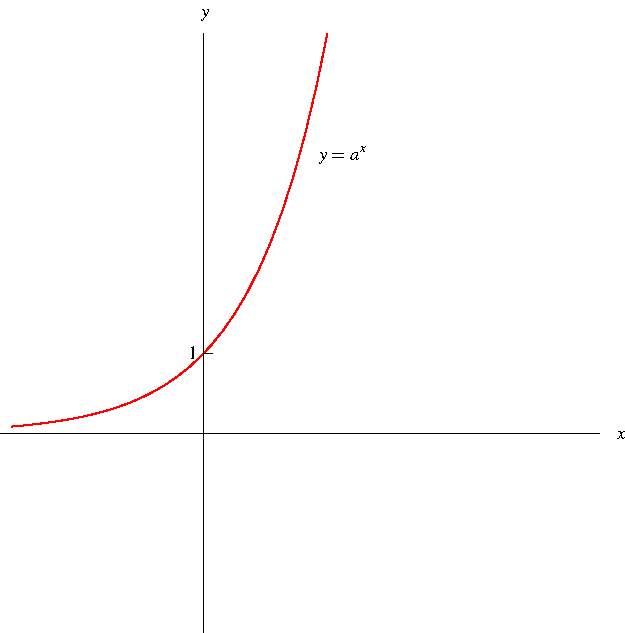
\includegraphics[height=4cm]{logarithms/pictures/07-03-logandexpa.pdf}%
%}%
%\only<8->{%
%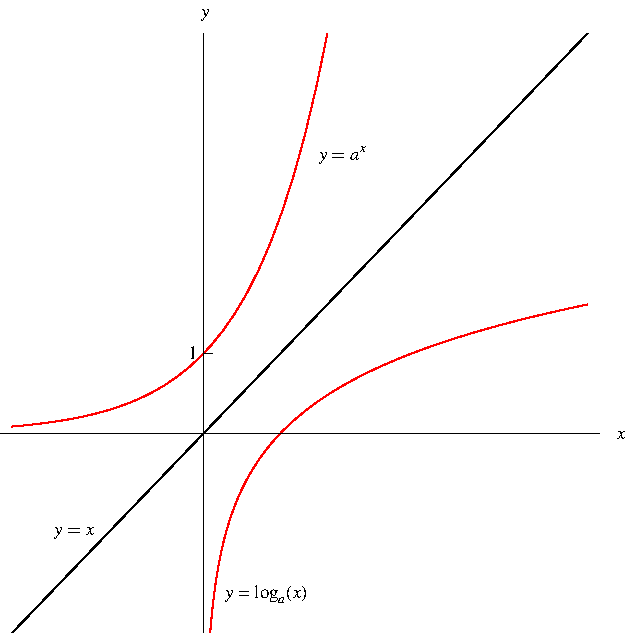
\includegraphics[height=4cm]{logarithms/pictures/07-03-logandexpb.pdf}%
%}%
\column{.7\textwidth}
\begin{itemize}
\item  Suppose $a > 0$, $a\neq 1$.
\item<2->  Let $f(x) = a^x$.
\item<3->  Then $f$ is either increasing or decreasing.
\item<4->  Therefore $f$ is one-to-one.
\item<5->  Therefore $f$ has an inverse function, $f^{-1}$.
\item<7->  The graph shows $y = a^x$ for $a > 1$.
\item<8->  The graph of $y = \log_a x$ is the reflection of this in the line $y = x$.
\end{itemize}
\end{columns}
\uncover<6->{%
\begin{definition}[$\log_a x$]
The inverse function of $f(x) = a^x$ is called the logarithmic function with base $a$, and is written $\log_a x$.  It is defined by the formula
\[
\log_a x = y \qquad \Leftrightarrow \qquad a^y = x .
\]
\end{definition}
}%
\end{frame}
% end module logarithm-def

% begin module logarithm-def-ex1
\begin{frame}
If $x > 0$, then $\log_a x$ is the exponent to which the base $a$ must be raised to give $x$.
\begin{example}%[Example 1, p. 405]
Evaluate:
\begin{enumerate}
\item<1-| alert@2-3> $\log_3 81 =$ \uncover<3->{$4$ because $3^4 = 81$.}
\item<1-| alert@4-5> $\log_{25} 5 =$ \uncover<5->{$\frac{1}{2}$ because $25^{1/2} = 5$.}
\item<1-| alert@6-7> $\log_{10} 0.001 =$ \uncover<7->{$-3$ because $10^{-3} = 0.001$.}
\end{enumerate}
\end{example}
\end{frame}
% end module logarithm-def-ex1

% begin module log-and-exp
\begin{frame}
\begin{columns}[c]
\column{.6\textwidth}
\psset{xunit=1cm, yunit=1cm}
\begin{pspicture}(-2,-2.1)(4.2, 4.2)
\psaxes[ticks=none, labels=none]{<->}(0,0)(-2,-2.1)(4.2, 4.2)
\psline(-0.1, 1)(0.1,1)
\rput[r](-0.2, 1){\footnotesize$1$}
\rput(0.9, 3){\footnotesize$y=a^x$}
%Function formula: 2^{x} 
\psplot[linecolor=red, plotpoints=1000]{-2}{2}{2 x exp }
\psplot[linecolor=red, plotpoints=1000]{0.25}{4}{x ln 0.693147181 div }
\psline[linestyle=dashed, linecolor=blue](-1.9, -1.9)(4,4) 
\rput[tl](2, 0.7){\footnotesize$y=\log_ax$}
\rput[tl](-1, -1.1){\footnotesize$y=x$}
\end{pspicture} 
%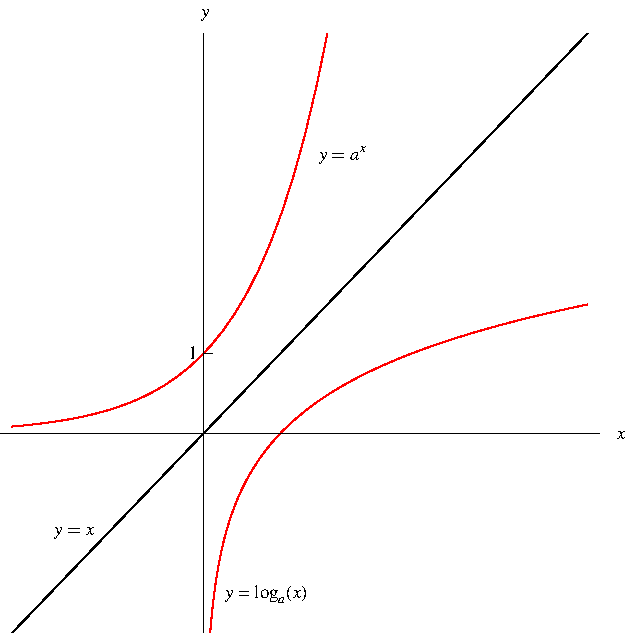
\includegraphics[height=7cm]{logarithms/pictures/07-03-logandexpb.pdf}%
\column{.4\textwidth}
\begin{itemize}
\item  Suppose $a > 1$.
\item<2-| alert@3-4>  Domain of $a^x$: \uncover<4->{$\mathbb{R}$.}
\item<2-| alert@5-6>  Range of $a^x$: \uncover<6->{$(0, \infty )$.}
\item<2-| alert@7-8>  Domain of $\log_a x$: \uncover<8->{$(0, \infty )$.}
\item<2-| alert@9-10>  Range of $\log_a x$: \uncover<10->{$\mathbb{R}$.}
\item<11->  $\log_a (a^x) = x$ for $x\in \mathbb{R}$.
\item<11->  $a^{\log_a x} = x$ for $x > 0$.
%\item<12-| alert@13-14>  $\lim_{x\rightarrow \infty}\log_a x = \uncover<14->{\infty .}$
%\item<12-| alert@15-16>  $\lim_{x\rightarrow 0^+}\log_a x = \uncover<16->{-\infty .}$
\end{itemize}
\end{columns}
\end{frame}
% end module log-and-exp

% begin module logarithm-graphs
\begin{frame}
\begin{center}
Graphs of various logarithmic functions with $a > 1$
\psset{xunit=1cm, yunit=1cm}
\begin{pspicture}(-5, -5)(5,5) 
\psframe*[linecolor=white](-5,-5)(5,5) 
\psaxes[ticks=none, labels=none]{<->}(0,0)(-0.5,-4.5)(7.5,2.5)
\psline(1,-0.1)(1,0.1)
%Function formula: ln(x)/ln(2)
\psplot[linecolor=red, plotpoints=1000]{0.044194174}{7.5}{x ln 0.693147181 div}
\rput[r](3, 1.8){\footnotesize $y=log_2 x$}
\uncover<2->{
%Function formula: ln{x}/ln(3) 
\psplot[linecolor=black, plotpoints=1000]{0.007127781}{7.5}{x ln 1.098612289 div}
\rput[l](3.6, 1.6 ){\footnotesize $y=log_3 x$}
}
\uncover<3->{
%Function formula: ln{x}/ln(5) 
\psplot[linecolor=blue, plotpoints=1000]{0.000715542}{7.5}{x ln 1.609437912 div}
\rput[l](3.7, 1.1){\footnotesize $y=log_5 x$}
}
\uncover<4->{
%Function formula: ln{x}/ln(5) 
\psplot[linecolor=green, plotpoints=1000]{0.000031623}{7.5}{x ln 2.302585093 div}
\rput[tl](3.6, 0.6){\footnotesize $y=log_{10} x$}
}
%\rput(6, 1){\color{red!1} .}
\end{pspicture} 
%\ \only<handout:0| -1>{%
%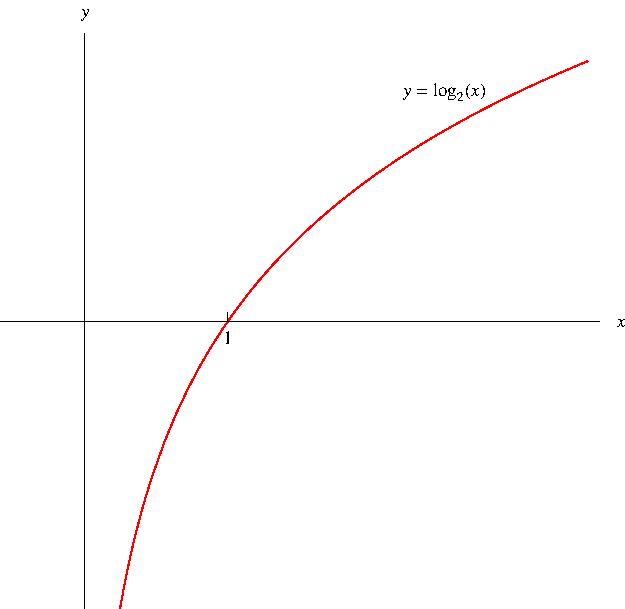
\includegraphics[height=6cm]{logarithms/pictures/07-03-manylogsa.pdf}%
%}%
%\only<handout:0| 2>{%
%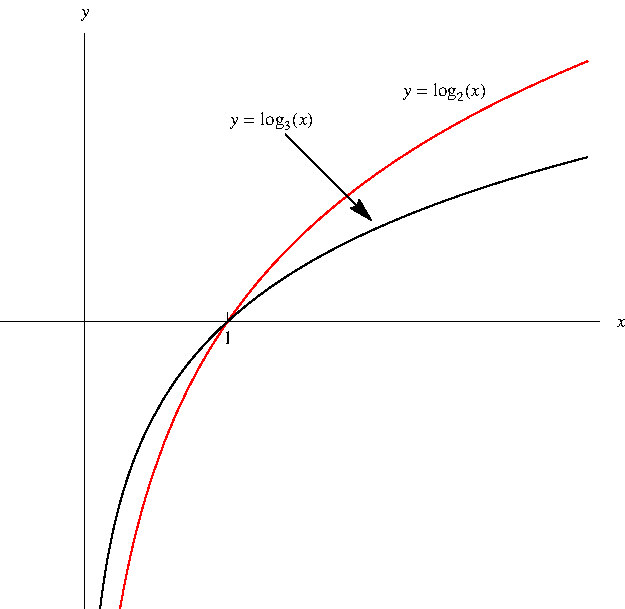
\includegraphics[height=6cm]{logarithms/pictures/07-03-manylogsb.pdf}%
%}%
%\only<handout:0| 3>{%
%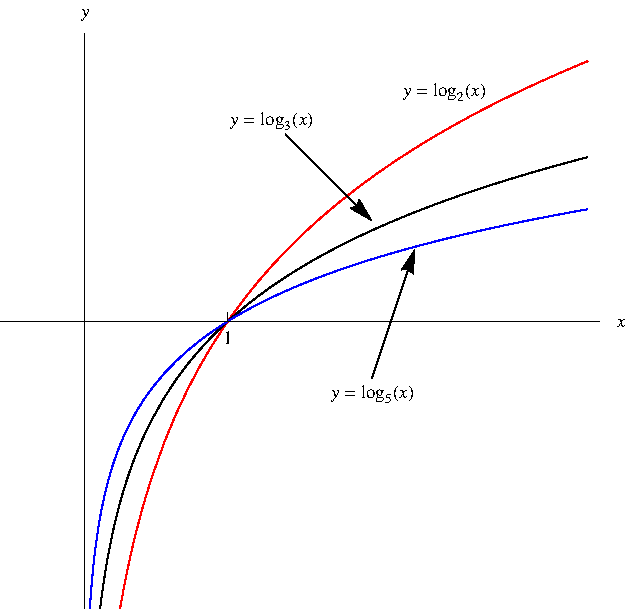
\includegraphics[height=6cm]{logarithms/pictures/07-03-manylogsc.pdf}%
%}%
%\only<4->{%
%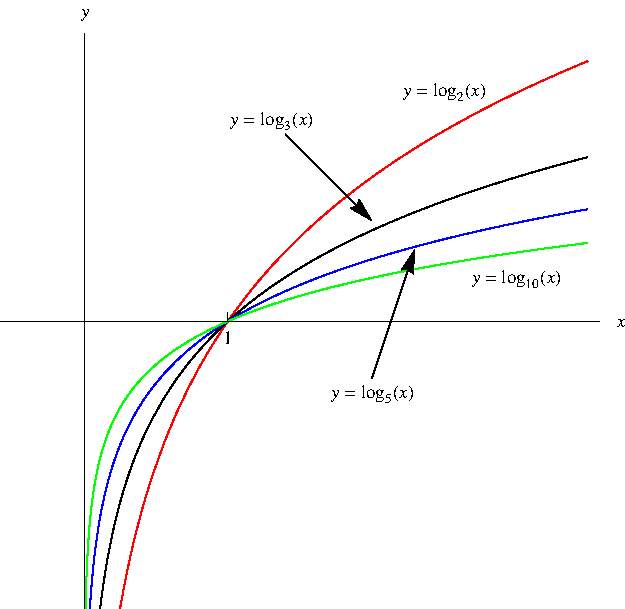
\includegraphics[height=6cm]{logarithms/pictures/07-03-manylogsd.pdf}%
%}%
\pause\pause\pause
\end{center}
\end{frame}
% end module logarithm-graphs
% begin module logarithm-properties
\begin{frame}
\begin{theorem}[Properties of Logarithmic Functions]
If $a > 1$, the function $f(x) = \log_a x$ is a one-to-one, continuous, increasing function with domain $(0, \infty )$ and range $\mathbb{R}$.  If $x, y, a, b > 0$ and $r$ is any real number, then
\begin{enumerate}
\item  $\log_a (xy) = \log_a x + \log_a y$.
\item  $\log_a \left( \frac{x}{y}\right) = \log_a x - \log_a y$.
\item  $\log_a (x^r) = r\log_a x$.
\item  $\log_{a}(x)=\log_b x \log_{a} b=\frac{\log_b x}{\log_{b} a}=  \frac{\ln x}{\ln a}$.
\end{enumerate}
\end{theorem}

\end{frame}
% end module logarithm-properties

% begin module logarithm-properties-ex2
\begin{frame}
\begin{example}
Use the properties of logarithms to evaluate the following:
\begin{columns}[t]
\column{.5\textwidth}
\begin{align*}
& \invisible{=} \log_{\alertNoH{2}{4}} \alertNoH{3}{2} + \log_{\alertNoH{2}{4}} \alertNoH{3}{32} \\
&\uncover<2->{=}  \uncover<2-| handout:0>{ \log_{ \alertNoH{2}{4}} (\alertNoH{4}{ \alertNoH{3}{2}\cdot \alertNoH{3}{32}} )} \\
&\uncover<4->{=}  \uncover<4-| handout:0>{ \alertNoH{5,6}{ \log_{ \alertNoH{7}{4}} (\alertNoH{4,9}{64})}} \\
&\uncover<5->{\alertNoH{5,6}{=}}  \fcAnswerNoH{6}{\alertNoH{8}{3}} \\
& \uncover<6-| handout:0>{\text{(because ${\alertNoH{7}{4}}^{\alertNoH{8}{3}} = \alertNoH{9}{64}$.)}}
\end{align*}
\column{.5\textwidth}
\begin{align*}
& \invisible{=} \log_{\alertNoH{10}{2}} 80 - \log_{ \alertNoH{10}{2} } 5 \\
&\uncover<10->{=}  \uncover<10-| handout:0>{ \log_{\alertNoH{10}{2}} \left(\alertNoH{11}{ \frac{80}{5}} \right) } \\
&\uncover<11->{=}  \uncover<11-| handout:0>{\alertNoH{12,13 }{ \log_{\alertNoH{14}{2}} (\alertNoH{11,16}{16})}} \\
&\uncover<12->{\alertNoH{12,13}{=}}  \fcAnswerNoH{13}{\alertNoH{15}{4}} \\
& \uncover<13-| handout:0>{\text{(because $\alertNoH{14}{2}^{\alertNoH{15}{4}} = \alertNoH{16}{16}$.)}}
\end{align*}
\end{columns}
\end{example}
\end{frame}
% end module logarithm-properties-ex2

\subsection{Natural Logarithms}
% begin module natural-logarithm-def
\begin{frame}
\frametitle{Natural Logarithms}
\begin{definition}[$\ln x$]
The logarithm with base $e$ is called the natural logarithm, and has a special notation:
\[
\log_e x = \ln x .
\]
\end{definition}
\begin{columns}[c]
\column{.5\textwidth}
\ 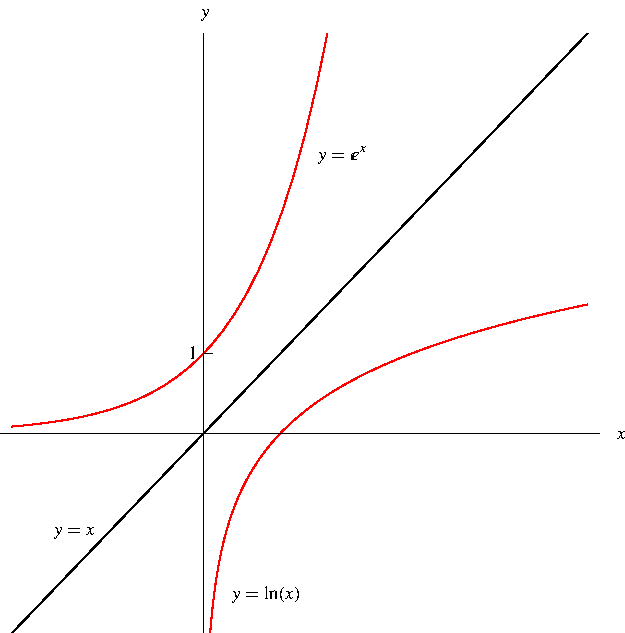
\includegraphics[height=5cm]{logarithms/pictures/07-03-natlog.pdf}%
\column{.5\textwidth}
\begin{itemize}
\item<2->  $\ln x = y \qquad \Leftrightarrow \qquad e^y = x$ .
\item<3->  $\ln (e^x ) = x$ for $x\in \mathbb{R}$.
\item<4->  $e^{\ln x}  = x$ for $x > 0$.
\end{itemize}
\end{columns}
\end{frame}
% end module natural-logarithm-def

% begin module natural-logarithm-def-ex5
\begin{frame}
\begin{example}
\begin{align*}
\text{Solve the equation} \quad e^{5-3x} & =  10 \\
\uncover<2-| handout:0>{\alertNoH{3}{\ln} ({\alertNoH{3}{e}}^{5-3x})} & \uncover<2->{=}  \uncover<2-| handout:0>{\ln 10} \\
\uncover<3-| handout:0>{\alertNoH{4}{5-}3x} & \uncover<3->{=}  \uncover<3-| handout:0>{\ln 10} \\
\uncover<4-| handout:0>{\alertNoH{5}{3}x} & \uncover<4->{=}  \uncover<4-| handout:0>{\alertNoH{4}{5-}\ln 10} \\
\uncover<5->{x} & \uncover<5->{=}  \uncover<5-| handout:0>{\frac{5-\ln 10}{\alertNoH{5}{3}}} \\
\uncover<6->{\text{Calculator:}\quad x} & \uncover<6->{\approx 0.8991.}
\end{align*}
\end{example}
\end{frame}
% end module natural-logarithm-def-ex5

% begin module exponential-equation3
\begin{frame}
\begin{columns}
\column{.55\textwidth}
\begin{example}[Finding the intersection of two exponential graphs]
Find the point(s) of intersection of $y = e^{2x}+4$ and $y = 5e^x$.  
\abovedisplayskip=0pt
\belowdisplayskip=0pt
\begin{align*}
\uncover<2->{ e^{2x} + 4 & = 5e^x }\\
\uncover<3-| handout:0>{\alert<handout:0| 5-6>{e^{2x}} - 5\alert<handout:0| 4>{e^x} + 4} & \uncover<3->{ = 0} \\
\intertext{\uncover<4->{Substitute $\alert<handout:0| 10>{u = \uncover<4-| handout:0>{e^x}}$:}}
\uncover<4-| handout:0>{\alert<handout:0| 5-6>{\uncover<6->{u^2}} - 5\alert<handout:0| 4>{u} + 4} & \uncover<4->{ = 0} \\
\uncover<7->{\alert<handout:0| 7-8>{(\uncover<8-| handout:0>{u-4})(\uncover<8-| handout:0>{u-1})}} & \uncover<7->{ = 0 } 
\end{align*}
\begin{align*}
\uncover<9->{ \alert<handout:0| 10>{u} } & \uncover<9->{=} \uncover<9-| handout:0>{ 4 } & \uncover<9->{\text{or}} & & \uncover<9->{\alert<handout:0| 10>{u}} & \uncover<9->{=} \uncover<9-| handout:0>{ 1} \\
\uncover<10-| handout:0>{ \alert<handout:0| 10>{e^x} } & \uncover<10-| handout:0>{ = 4 } & \uncover<10-| handout:0>{\text{or}} & & \uncover<10-| handout:0>{\alert<handout:0| 10>{e^x}} & \uncover<10-| handout:0>{ = 1} \invisible{99999999} \\
\uncover<11-| handout:0>{ \alert<handout:0| 11-12>{x} } & \uncover<11-| handout:0>{ \alert<handout:0| 11-12>{ = \uncover<12->{\ln 4} }} & \uncover<11-| handout:0>{\text{or}} & & \uncover<11-| handout:0>{\alert<handout:0| 13-14>{x}} & \uncover<11-| handout:0>{ \alert<handout:0| 13-14>{ = \uncover<14->{0} }} 
\end{align*}
\uncover<15-19| handout:0>{Therefore the points of intersection are \alert<handout:0| 15-16>{$(\ln 4,\uncover<16->{20})$} and \alert<handout:0| 17-18>{$(0,\uncover<18->{5})$}.}  
\end{example}

\column{.4\textwidth}

\uncover<19-| handout:0>{%
\psset{xunit=0.3cm,yunit=0.13cm,algebraic=true,dotstyle=o,dotsize=3pt 0,linewidth=0.8pt,arrowsize=3pt 2,arrowinset=0.25}
\begin{pspicture*}(-6.92,-4.61)(9.16,53.92)
\psaxes[labelFontSize=\scriptstyle,xAxis=true,yAxis=true,Dx=5,Dy=5,ticksize=-2pt 0,subticks=0]{<->}(0,0)(-6.92,-4.61)(9.16,53.92)
\psplot[linecolor=blue,plotpoints=200]{-6.915925925925918}{9.164074074074078}{5*EXP(x)}
\psplot[linecolor=red,plotpoints=200]{-6.915925925925918}{9.164074074074078}{EXP(2*x)+4}
\begin{scriptsize}
\rput[tl](2.6,40.0){$y=5e^x$}
\rput[tl](-7.0,6.5){$y=e^x+4$}
\psdots[dotstyle=*](0,5)
\rput[bl](0.1,3.99){$(0, 5)$}
\psdots[dotstyle=*](1.39,20)
\rput[bl](1.46,18.52){$(\ln4,20)$}
\end{scriptsize}
\end{pspicture*}
}%

\end{columns}
\end{frame}
% end module exponential-equation3

% begin module exponential-equation4
\begin{frame}
\begin{example}[Solving a quadratic exponential equation]
Solve for $x$.  
\abovedisplayskip=0pt
\belowdisplayskip=0pt
\begin{align*}
4^{x+1} & = 2^{x+2} + 3 \\
\uncover<2-| handout:0>{\alert<handout:0| 6>{4^{x+1}} - \alert<handout:0| 4>{2^{x+2}} - 3} & \uncover<2->{ = 0} \\
\intertext{\uncover<3->{Substitute $\alert<handout:0| 10>{u = \uncover<3-| handout:0>{2^x}}$.  Then $\alert<handout:0| 3-4>{2^{x+2} = \uncover<4-| handout:0>{4u}}$ and $\alert<handout:0| 5-6>{4^{x+1} = \uncover<6-| handout:0>{4u^2.}}$ }}
\uncover<3-| handout:0>{\alert<handout:0| 6>{\uncover<6->{4u^2}} - \alert<handout:0| 4>{\uncover<4->{4u}} - 3} & \uncover<3->{ = 0} \\
\uncover<7->{\alert<handout:0| 7-8>{(\uncover<8-| handout:0>{2u-3})(\uncover<8-| handout:0>{2u+1})}} & \uncover<7->{ = 0 } 
\end{align*}
\begin{align*}
\uncover<9->{ \alert<handout:0| 10>{u} } & \uncover<9->{=} \uncover<9-| handout:0>{ \frac{3}{2} } & \uncover<9->{\text{or}} & & \uncover<9->{\alert<handout:0| 10>{u}} & \uncover<9->{=} \uncover<9-| handout:0>{ -\frac{1}{2}} \\
\uncover<10-| handout:0>{ \alert<handout:0| 10>{2^x} } & \uncover<10-| handout:0>{ = \frac{3}{2} } & \uncover<10-| handout:0>{\text{or}} & & \uncover<10-| handout:0>{\alert<handout:0| 10>{2^x}} & \uncover<10-| handout:0>{ = -\frac{1}{2}} \invisible{99999999} \\
\uncover<11-| handout:0>{ \alert<handout:0| 11-12>{x} } & \uncover<11-| handout:0>{ \alert<handout:0| 11-12>{ = \uncover<12->{\log_2 \Big( \frac{3}{2}\Big)} }} & & & \uncover<11-| handout:0>{\alert<handout:0| 13-14>{\uncover<-13>{x}}} & \uncover<11-| handout:0>{ \alert<handout:0| 13-14>{ \only<-13>{ =} \only<14->{\text{no solution}} }} \\
\uncover<15-| handout:0>{x & = \frac{\ln (3/2)}{\ln2} & & & & } 
\end{align*}
\uncover<16-| handout:0>{Therefore the solution is $x = \frac{\ln (3/2)}{\ln 2} \approx  0.584962501$.}
\end{example}
\end{frame}
% end module exponential-equation4

% begin module natural-logarithm-def-ex8
\begin{frame}
\begin{example}%[Example 8, p. 408]
Draw the graph of $y = \ln (x - 2) -1$.
\ \only<handout:0| -1>{%
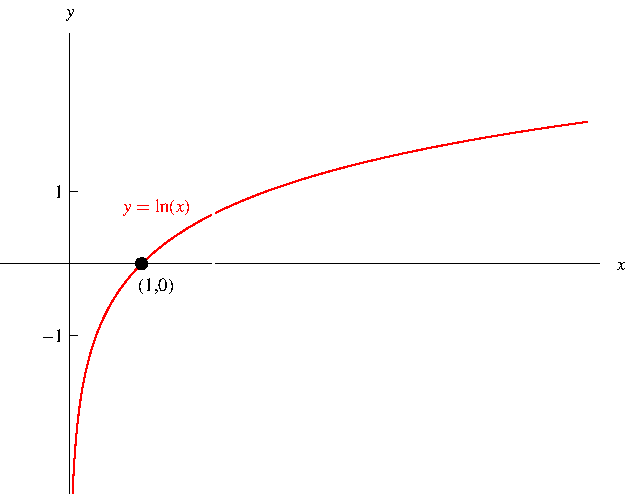
\includegraphics[height=6cm]{logarithms/pictures/07-03-ex8a.pdf}%
}%
\only<handout:0| 2>{%
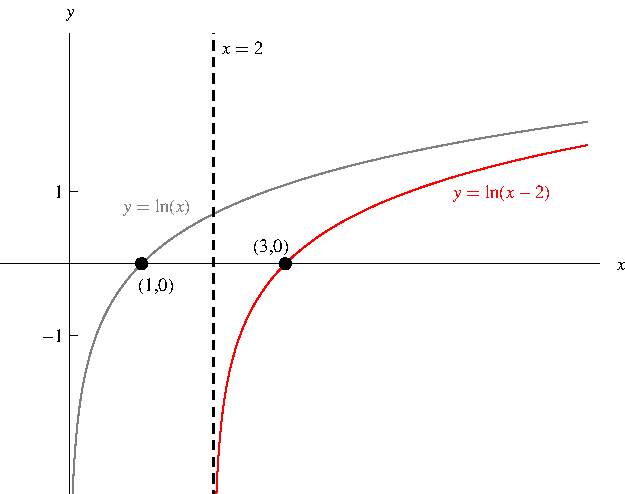
\includegraphics[height=6cm]{logarithms/pictures/07-03-ex8b.pdf}%
}%
\only<3->{%
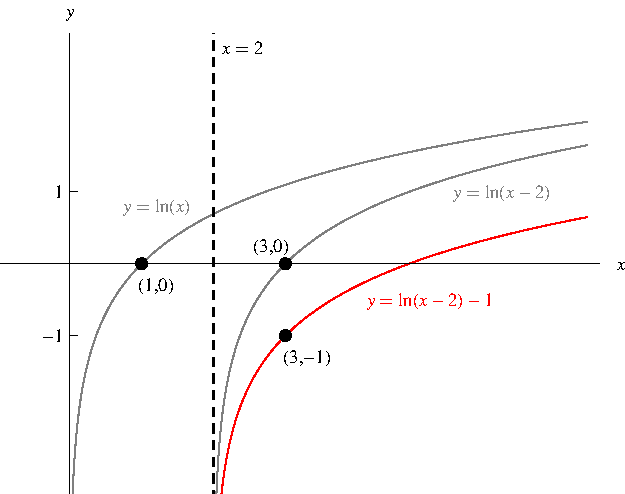
\includegraphics[height=6cm]{logarithms/pictures/07-03-ex8c.pdf}%
}%
\end{example}
\end{frame}
% end module natural-logarithm-def-ex8

% begin module inverse-function-solve-for
\begin{frame}
%\frametitle{Inverse of a ne-to-one Function}
\begin{example}
Given: $f(x) = \frac{e^x-e^{-x}}{e^x+e^{-x}}  $.  Find $f^{-1}(x)$.
\begin{columns}
\column{0.4\textwidth}
\psset{xunit=0.8cm, yunit=0.8cm}
\begin{pspicture}(-3.05,-3.1)(3.15,3.2)
\psframe*[linecolor=white](-3.05,-3.1)(3.15,3.2)
\tiny
\psaxes[ticks=none, labels=none]{<->}(0,0)(-3.05,-3.1)(3.05,3.1)
\fcLabels{3.05}{3.1}
%Function formula: (679570457/250000000^{x}- (679570457/250000000^{- (x)}))/(679570457/250000000^{- (x)}+679570457/250000000^{x})
\uncover<1-14>{
\rput(-2,-0.5){$y=f(x)$}
\psplot[linecolor=\fcColorGraph, plotpoints=1000]{-3}{3}{2.71828 x -1 mul exp -1 mul 2.71828 x exp add 2.71828 x exp 2.71828 x -1 mul exp add div }
}
\uncover<15->{
\rput(-2,-0.5){$y=f(x)$}
\psplot[linecolor=gray!50, plotpoints=1000]{-3}{3}{2.71828 x -1 mul exp -1 mul 2.71828 x exp add 2.71828 x exp 2.71828 x -1 mul exp add div }
}
%Function formula: 1/2 (\ln{}((1+x)/(1- (x))))
\uncover<15->{
\rput[tl](1.1,2.5){$y=f^{-1}(x)$}
\psplot[linecolor=\fcColorGraph, plotpoints=1000]{-0.994}{0.994}{x 1 add x -1 mul 1 add div ln 0.5 mul }
}
\end{pspicture}
\uncover<15->{Final }\uncover<14->{answer}\uncover<15->{, \alert<15>{relabelled}:}
\[
\uncover<14->{
f^{-1}( \only<14>{y}\only<15->{\alert<15>{x}} )=\frac12\ln\frac{1+\only<14>{y}\only<15->{\alert<15>{x}} }{1-\only<14>{y}\only<15->{\alert<15>{x}}}
}
\]
\column{0.6\textwidth}
\uncover<2->{Set $u=e^x$.} \uncover<3->{Then $\alert<3>{e^{-x}=} \uncover<4->{\alert<4>{\frac1u}}$.}
\[\begin{array}{rcl}
\uncover<5->{ \frac{u-\frac1u}{u+\frac1u}&=&y}\\
\uncover<6->{\frac{u^2-1}{u^2+1}&=&y}\\
\uncover<7->{u^2-1&=&y(u^2+1)}\\
\uncover<8->{u^2(1-y)&=&1+y}\\
\uncover<9->{u^2&=&\frac{1+y}{1-y}}\\
\uncover<10->{u&=& \only<10>{\pm}\only<11>{\alert<11>{+}} \sqrt{\frac{1+y}{1-y}}}\\
\uncover<12->{\uncover<13->{x=\ln e^x =}\alert<12>{\ln} u &=& \alert<12>{\ln}\sqrt{\frac{1+y}{1-y}}}\uncover<14->{=\frac12\ln\frac{1+y}{1-y}} \\
\end{array}
\]
\uncover<11->{where the sign follows from $e^x=u>0$.} \uncover<12->{Take $\alert<12>{\ln} $ on both sides.}
\end{columns}
\end{example}
\end{frame}
% end module inverse-function-solve-for

% end lecture

% begin lecture
\lect{February 28, 2014}{Lecture 10}{10}
\section{Implicit Differentiation}
% begin module implicit-differentiation-intro
\begin{frame}
\frametitle{Implicit Differentiation}
\begin{itemize}
\item  So far, we have seen functions with formulas that express one varable explicitly in terms of the other.
\item<2->  $y = \sqrt{x^3+1}$, $y = x\sin x$, etc.
\item<3->  Some functions are given implicitly by a relation between $x$ and $y$.
\item<4->  $x^2 + y^2 = 1$ isn't the equation of any one function.
\item<5->  Implicitly it gives two functions: \uncover<6->{$\alert<6>{y = \sqrt{1-x^2}}$ and} \uncover<7->{\alert<7>{$ y = -\sqrt{1-x^2}$}.}
\item<8->  How do we differentiate these functions?
\item<9->  Differentiate both sides with respect to $x$, and then solve for $y'$.
\end{itemize}
\begin{center}
\psset{xunit=1.5cm, yunit=1.5cm}
\begin{pspicture}(-1.8, -1.15)(1.8,1.25)
\tiny
\psaxes[ticks=none, labels=none]{<->}(0,0)(-1.7,-1.15)(1.7,1.2)
\fcLabels{1.7}{1.2}
\uncover<4,5,6,8->{
\psplot[linecolor=\fcColorGraph, plotpoints=1000]{-1}{1}{x 2 exp -1 mul 1 add sqrt }
}
\uncover<7>{
\psplot[linestyle=dashed, linecolor=gray!50, plotpoints=1000]{-1}{1}{x 2 exp -1 mul 1 add sqrt }
}
\uncover<4,5,7,8->{
\psplot[linecolor=\fcColorGraph, plotpoints=1000]{-1}{1}{x 2 exp -1 mul 1 add sqrt -1 mul }
}
\uncover<6>{
\psplot[linestyle=dashed, linecolor=gray!50, plotpoints=1000]{-1}{1}{x 2 exp -1 mul 1 add sqrt -1 mul }
}
\uncover<6->{\rput[l](0.5,1){$y=\sqrt{1- x^{2}}$} }
\uncover<7->{\rput[l](0.5,-1){$y=- \sqrt{1- x^{2}}$} }
\end{pspicture}

%\ \uncover<5->{%
%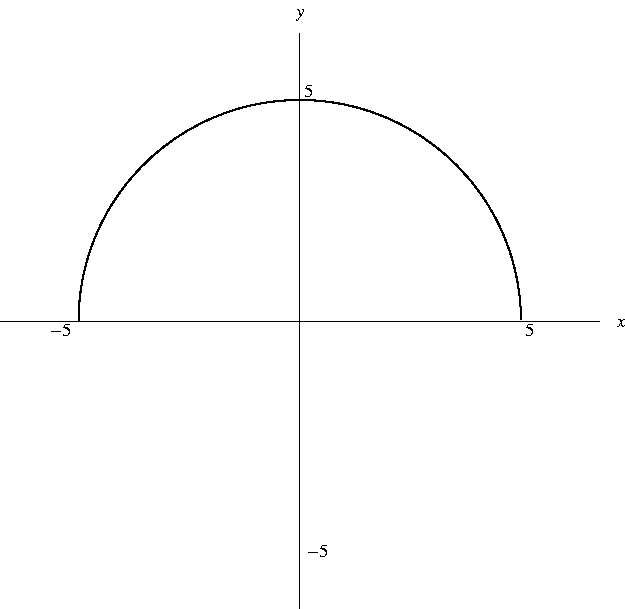
\includegraphics[height=2.5cm]{implicit-differentiation/pictures/03-06-circletop.pdf}%
%}%
%\ \uncover<4->{%
%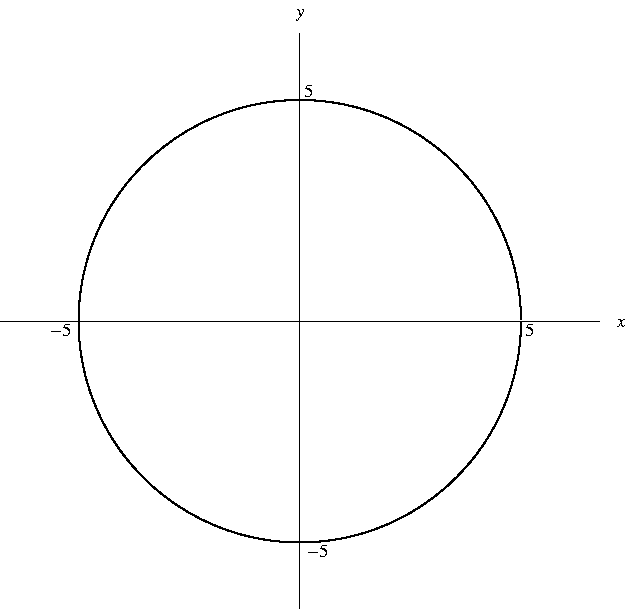
\includegraphics[height=2.5cm]{implicit-differentiation/pictures/03-06-circle.pdf}%
%}%
%\ \uncover<5->{%
%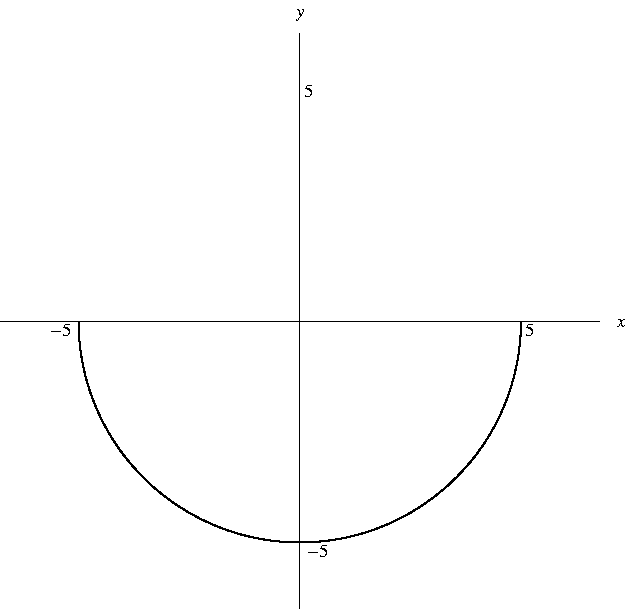
\includegraphics[height=2.5cm]{implicit-differentiation/pictures/03-06-circlebottom.pdf}%
%}%
\end{center}
\end{frame}
% end module implicit-differentiation-intro

% begin module implicit-tangent-line
\abovedisplayskip=0pt
\belowdisplayskip=0pt
\abovedisplayshortskip=0pt
\belowdisplayshortskip=0pt
\begin{frame}
\begin{example}
Find an equation of the tangent line to $(x-1)^2 + (y+2)^2 = 25$ at $(-2,2)$.
\begin{columns}
\column{1.2in}
\begin{center}
\only<handout:0|-15>{\includegraphics[height=3cm]{implicit-differentiation/pictures/implicit-tangent-line(a).jpg}}
\only<16->{\includegraphics[height=3cm]{implicit-differentiation/pictures/implicit-tangent-line(b).jpg}}
\end{center}
\begin{align*}
\uncover<15->{&\text{Plug in} \ (-2,2):}\\
\uncover<15->{&\frac{\diff y}{\diff x}  = \frac{1+2}{4} = \frac{3}{4}}\\
\uncover<16->{&\text{Point-slope form:}\\
&y-2 = \frac{3}{4} (x+2)}
\end{align*}
\column{3in}
\abovedisplayskip=0pt
\belowdisplayskip=0pt
\abovedisplayshortskip=0pt
\belowdisplayshortskip=0pt
\begin{align*}
\uncover<2->{\text{Find} \ \frac{\diff y}{\diff x}, \ \text{given} \ (x-1)^2 \ + (y+2)^2 & = 25:} \\
\uncover<3->{\alert<handout:0|3-4>{\frac{\diff}{\diff x}\left((x-1)^2\right)} + \alert<handout:0|5-6>{\frac{\diff}{\diff x}\left((y+2)^2\right)}   &= \alert<handout:0|7-8>{\frac{\diff}{\diff x}(25)}}\\
\uncover<3->{\uncover<4->{\alert<handout:0|4>{2(x-1)\alert<handout:0|9>{\frac{\diff}{\diff x}(x-1)}}} +\uncover<6->{\alert<handout:0|6>{ 2(y+2)\alert<handout:0|11-12>{\frac{\diff}{\diff x}(y+2) }}}  &= \uncover<8->{\alert<handout:0|8>{0}}}\\
\uncover<9->{2(x-1)\alert<handout:0|9-10> {(\uncover<10>{1})}+ 2(y+2)\alert<handout:0|11-12>{\left( \uncover<12->{\frac{\diff y}{\diff x}} \right)}  & = 0}\\
\uncover<13->{2(y+2)\left( \frac{\diff y}{\diff x} \right) & = -2(x-1)}\\
\uncover<14->{\frac{\diff y}{\diff x} &=  \frac{1-x}{y+2}}
\end{align*}
\end{columns}
\end{example}
\end{frame}
% end module implicit-tangent-line
% begin module implicit-differentiation-ex3
\begin{frame}
\begin{example}[Example 3, p. 213]
\abovedisplayskip=0pt
\belowdisplayskip=-15pt
\abovedisplayshortskip=0pt
\belowdisplayshortskip=0pt
\begin{align*}
\text{Find $y'$ if }\sin (x+y) & = y^2\cos x.\\
\uncover<2->{%
\alert<handout:0| 3-4>{\frac{\diff}{\diff x} (\sin (x+y))}%
}%
& \uncover<2->{ = } %
\uncover<2->{%
\alert<handout:0| 5-6>{\frac{\diff}{\diff x} (y^2\cos x)}%
}\\%
\uncover<4->{%
\alert<handout:0| 3-4>{(\cos(x+y))\alert<handout:0| 7-8>{\frac{\diff}{\diff x}(x+y)}}%
}%
& \uncover<3->{ = } %
\uncover<6->{%
\alert<handout:0| 5-6>{(y^2)\alert<handout:0| 9-10>{\frac{\diff}{\diff x}(\cos x)} + (\cos x) \alert<handout:0| 11-12>{\frac{\diff}{\diff x}(y^2)}}%
}\\%
\uncover<7->{%
(\cos(x+y))\alert<handout:0| 7-8>{\left(\uncover<8->{1+y'}\right)}%
}%
& \uncover<7->{ = } %
\uncover<7->{%
(y^2)\alert<handout:0| 9-10>{(\uncover<10->{-\sin x})} + (\cos x) \alert<handout:0| 11-12>{(\uncover<12->{2yy'})}%
}\\%
\uncover<13->{%
\cos(x+y) + y'\cos(x+y)%
}%
& \uncover<13->{ = %
-y^2\sin x +2yy'\cos x%
}\\%
\uncover<14->{%
\alert<handout:0| 15>{y'}\cos(x+y) - 2y\alert<handout:0| 15>{y'}\cos x%
}%
& \uncover<14->{ = %
-y^2\sin x -\cos(x+y)%
}\\%
\uncover<15->{%
\text{Factor:}\quad%
\alert<handout:0| 15>{y'}(\cos(x+y) - 2y\cos x)%
}%
& \uncover<15->{ = %
-y^2\sin x -\cos(x+y)%
}\\%
\uncover<16->{%
y'%
}%
& \uncover<16->{ = } %
\uncover<16->{%
\frac{-y^2\sin x - \cos(x+y)}{\cos (x+y) - 2y\cos x}.%
}%
\end{align*}
\end{example}
\end{frame}
% end module implicit-differentiation-ex3

% begin module implicit-trig
\begin{frame}
\begin{example}[Implicit Differentiation]
\abovedisplayskip=0pt
\belowdisplayskip=-15pt
\abovedisplayshortskip=0pt
\belowdisplayshortskip=0pt
\begin{align*}
\text{Find $y'$ if } \tan xy &= x^2-y^2.\\
\uncover<2->{\alert<handout:0|3-4>{\frac{\diff}{\diff x}(\tan xy)}&= \alert<handout:0|5-6>{ \frac{\diff}{\diff x}(x^2-y^2)}}\\
\uncover<3->{\alert<handout:0|4>{\uncover<4->{(\sec^2xy)\alert<handout:0|7-8>{\frac{\diff}{\diff x}(xy)}}} & = \uncover<6->{\alert<handout:0|6>{ 2x-2yy'}}}\\
\uncover<7->{\alert<handout:0|7-8>{\left(\uncover<8->{y\alert<handout:0|9-10>{\frac{\diff}{\diff x}(x)}+x\alert<handout:0|11-12>{\frac{\diff}{\diff x}(y)}}\right)}\sec^2 xy &= 2x -2yy'}\\
\uncover<9->{\left(y\alert<handout:0|9-10>{(\uncover<10->{1})}+x\alert<handout:0|11-12>{(\uncover<12->{y'})}\right)\sec^2 xy &= 2x -2yy'}\\
\uncover<13->{y\sec^2xy+xy' \sec^2xy &= 2x -2yy'}\\
\uncover<14->{xy' \sec^2xy+2yy'&=2x-y\sec^2xy}\\
\uncover<15->{y'(x\sec^2xy+2y) &= 2x-y\sec^2xy}\\
\uncover<16->{y'&=\frac{2x-y\sec^2xy}{x\sec^2xy+2y}.}
\end{align*}
\end{example}
\end{frame}
% end module implicit-trig

% begin module implicit-differentiation-ex4
\begin{frame}
\begin{example}[Example 4, p. 213]
%\uncover<2->{Differentiate implicitly:}%
\abovedisplayskip=0pt
\belowdisplayskip=0pt
\abovedisplayshortskip=0pt
\belowdisplayshortskip=0pt
\begin{align*}
\text{Find $y''$ if } \alert<handout:0| 14>{x^4 + y^4} & \alert<handout:0| 14>{ = 16}. \\
\uncover<2->{%
4x^3 + 4y^3y'%
}%
& \uncover<2->{ = } %
\uncover<2->{%
0%
}\\%
\uncover<3->{%
\alert<handout:0| 10>{y'}%
}%
& \uncover<3->{ \alert<handout:0| 10>{=} } %
\uncover<3->{%
\alert<handout:0| 10>{-\frac{x^3}{y^3}}.%
}\\%
\uncover<4->{%
y''%
}%
& \uncover<4->{ = } %
\uncover<4->{%
\frac{\diff}{\diff x}\left( -\frac{x^3}{y^3}\right)%
}  \uncover<5->{ = } %
\uncover<5->{%
- \frac{y^3 \alert<handout:0| 6-7>{\frac{\diff}{\diff x}(x^3)} - x^3\alert<handout:0| 8-9>{\frac{\diff}{\diff x}(y^3)}}{(y^3)^2}%
}\\%
& \uncover<6->{ = } %
\uncover<6->{%
- \frac{y^3 (\alert<handout:0| 6-7>{\uncover<7->{3x^2}}) - x^3(\alert<handout:0| 8-9>{\uncover<9->{3y^2\alert<handout:0| 10>{y'}}})}{y^6}%
} \uncover<10->{ = }%
\uncover<10->{%
- \frac{3x^2y^3  - 3x^3y^2\alert<handout:0| 10>{\left( -\frac{x^3}{y^3}\right)}}{y^6}%
}\\%
& \uncover<11->{ = } %
\uncover<11->{%
- \frac{3x^2(y^3+\frac{x^4}{y})}{y^6}%
} \uncover<12->{ = }%
\uncover<12->{%
- \frac{3x^2\left( \frac{y^4+x^4}{\alert<handout:0| 13>{y}}\right)}{\alert<handout:0| 13>{y^6}}%
}\\%
& \uncover<13->{ = } %
\uncover<13->{%
- \frac{3x^2(\alert<handout:0| 14>{y^4+x^4})}{\alert<handout:0| 13>{y^7}}%
}  \uncover<14->{ = }%
\uncover<14->{%
- \frac{3x^2(\alert<handout:0| 14>{16})}{y^7}%
} \uncover<15->{ = }%
\uncover<15->{%
-48 \frac{x^2}{y^7}.%
}%
\end{align*}
\end{example}
\end{frame}
% end module implicit-differentiation-ex4

%\input{../../modules/implicit-differentiation/implicit-second-derivative}
% end lecture

% begin lecture
\lect{March 7, 2014}{Lecture 12}{12}
\section{Derivatives of Logarithmic and Exponential Functions}
\subsection{Derivatives of Logarithmic Functions}
% begin module general-log-derivative-implicit
\begin{frame}
\frametitle{Derivatives of Logarithmic Functions}
\begin{theorem}[The Derivative of $\log_a x$]
\[
\frac{\diff}{\diff x} (\log_a x) = \frac{1}{x\ln a} .
\]
\end{theorem}
\begin{proof}
\abovedisplayskip=0pt
\belowdisplayskip=0pt
\abovedisplayshortskip=0pt
\belowdisplayshortskip=0pt
\begin{align*}
\uncover<2->{%
\text{Let } y %
}%
& \uncover<2->{%
 = \log_a x. %
}\\%
\uncover<3->{%
\text{Then } \alertNoH{ 4-5,9}{a^y} %
}%
& \uncover<3->{%
 \alertNoH{ 9}{=} \alertNoH{ 6-7,9}{x}. %
}\\%
\uncover<4->{%
\text{Differentiate implicitly:}\quad \alertNoH{ 4-5}{\fcAnswer{5}{a^y (\ln a) y'}} %
}%
& \uncover<4->{%
 = \alertNoH{ 6-7}{\fcAnswerUncover{4}{7}{1}} %
}\\%
\uncover<8->{%
y' %
}%
& \uncover<8->{%
 = \frac{1}{\alertNoH{ 9}{a^y}\ln a} %
}\\%
& \uncover<9->{%
 = \frac{1}{\alertNoH{ 9}{x}\ln a}. %
}%
\end{align*}
\end{proof}
\end{frame}
% end module general-log-derivative-implicit

% begin module general-log-derivative-ex.tex
\begin{frame}
\chainrulefofx{\log_3(5^{x}+1)}{5^x+1}{\log_3 x}{\frac{1}{ UU \ln 3}}{5^x \ln 5 }{\frac{5^x \ln 5}{(5^x+1) \ln 3}}{0}
\end{frame}
% end module general-log-derivative-ex.tex
% begin module natural-log-derivative-from-general
\begin{frame}
\begin{theorem}[The Derivative of $\log_a x$]
\[
\frac{\diff}{\diff x} (\log_a x) = \frac{1}{x\ln a} .
\]
\end{theorem}

$\ln x = \log_e x$. Therefore when we set $a = e$ we get the derivative of $\ln x$:
\begin{align*}
\frac{\diff}{\diff x}(\ln x) & = \frac{1}{x\alertNoH{ 2-3}{\ln e}} \\
 & \uncover<2->{= \frac{1}{x\alertNoH{2-3}{( \fcAnswer{3}{1}) }}} \\
 & \uncover<4->{= \frac{1}{x}.}
\end{align*}
\uncover<5->{%
\begin{theorem}[The Derivative of $\ln x$]
\[
\frac{\diff}{\diff x} (\ln x) = \frac{1}{x}.
\]
\end{theorem}
}%
\end{frame}
% end module natural-log-derivative-from-general

% begin module natural-log-derivative-ex-simplify.tex
\begin{frame}
\begin{example}[Chain Rule, Natural Logarithm]
\abovedisplayskip=0pt
\belowdisplayskip=0pt
\abovedisplayshortskip=0pt
\belowdisplayshortskip=0pt
\begin{align*}
\text{Differentiate}\quad y &= \ln (e^x \sec x).\\
\uncover<2->{ y&= \alert<handout:0|3-4>{\ln e^x} + \ln \sec x}\\
\uncover<3->{ &=\uncover<4->{\alert<handout:0|4>{\alert<handout:0|5-6>{ x}}} + \ln \sec x.}\\
\uncover<5->{\frac{\diff y}{\diff x} & =\uncover<6->{\alert<handout:0|6>{1} }+ \uncover<7->{ \alert<handout:0|7>{\alert<handout:0|11>{\frac{\diff}{\diff x} (\ln \sec x)}}}}\\
\uncover<8->{\alert<handout:0|8-9>{\text{Let} \ \ \alert<handout:0|14-16>{u} }&  \alert<handout:0|8-9>{\alert<handout:0|14-16>{= \uncover<9->{ \sec x.}}}}\\
\uncover<10->{\text{Then} \ \ \ln \sec x & = { \ln u}.}\\
\uncover<11->{\text{Chain Rule:} \quad \frac{\diff y}{\diff x} & = 1+  \alert<handout:0|11>{\alert<handout:0|12-13>{\frac{\diff}{\diff u}(\ln u)} \alert<handout:0|14-15>{\frac{\diff u}{\diff x}}}}\\
\uncover<12->{& = 1+ \alert<handout:0|12-13>{\left( \uncover<13->{\frac{1}{\alert<handout:0|16>{u}}} \right)} \alert<handout:0|14-15>{(\uncover<15->{\sec x \tan x} )} }\\
\uncover<16->{& = 1+ \frac{1}{\alert<handout:0|16>{\sec x}}\sec x \tan x} \\
\uncover<17->{& = 1+ \tan x.}
\end{align*}
\end{example}
\end{frame}
% begin module natural-log-derivative-ex-simplify.tex
% begin module natural-logarithm-derivative-ex7
\begin{frame}
\begin{example}
\abovedisplayskip=0pt
\belowdisplayskip=0pt
\abovedisplayshortskip=0pt
\belowdisplayshortskip=0pt
\begin{align*}
\text{Find $f'(x)$ if } f(x) & = \ln |x|.\\
\uncover<2->{%
f(x) %
}% 
& \uncover<2->{
 = \left\{ \begin{array}{lr}
\alert<handout:0| 3-4>{\ln x} & \text{ if } x > 0 \\
\alert<handout:0| 5-6>{\ln (-x)} & \text{ if } x < 0 \\
\end{array}\right. .
}\\%
\uncover<3->{%
f'(x) %
}%
& \uncover<3->{
 = \left\{ \begin{array}{lr}
\alert<handout:0| 3-4>{\uncover<4->{\frac{1}{x}}} & \text{ if } x > 0 \\
\alert<handout:0| 5-6>{\uncover<6->{\frac{1}{-x}(-1)}} & \text{ if } x < 0 \\
\end{array}\right.
}\\%
& \uncover<7->{
 = \left\{ \begin{array}{lr}
\frac{1}{x} & \text{ if } x > 0 \\
\frac{1}{x} & \text{ if } x < 0 \\
\end{array}\right.
}\\%
& \uncover<8->{%
 = \frac{1}{x} \text{ if } x \neq 0.
}%
\end{align*}
\end{example}
\end{frame}
% end module natural-logarithm-derivative-ex7

\subsection{Derivatives of General Exponential Functions}
% begin module chain-rule-general-exponential.tex
\begin{frame}
\begin{example}[Chain Rule, general exponential function]
\begin{align*}
\text{Differentiate}\quad y & = \alert<handout:0|2-3>{2}^x.\\
\uncover<2->{y} & \uncover<2->{= \alert<handout:0|2-3>{( e^{\uncover<3->{\ln 2}} )}^x}\\
\uncover<4->{y} & \uncover<4->{= e^{x\ln 2}.}\\
\uncover<5->{\text{Let} \quad \alert<handout:0|5-6>{\alert<handout:0|13-14>{\alert<handout:0|11-12>{u}}} &\alert<handout:0|5-6>{\alert<handout:0|11-14>{=}} \uncover<6->{\alert<handout:0|6>{\alert<handout:0|11-12>{\alert<handout:0|13-14>{ x\ln 2.}}}}} \\
\uncover<7->{\text{Then} \quad \alert<handout:0|9-10>{y} &\alert<handout:0|9-10>{= e^u.}} \\
\uncover<8->{\text{Chain Rule:}\quad \frac{\diff y}{\diff x} &= \alert<handout:0|9-10>{ \frac{\diff y}{\diff u}}\alert<handout:0|11-12>{ \frac{\diff u}{\diff x}}}\\
\uncover<9->{&= \alert<handout:0|9-10>{(\uncover<10->{e^{\alert<handout:0|13-14>{u}}})}\alert<handout:0|11-12>{(\uncover<12->{\ln 2})} }\\
\uncover<13->{ &= (e^{\alert<handout:0|13-14>{(\uncover<14->{x\ln2})}})(\ln 2)}\\
\uncover<15->{& = (2^x)(\ln 2)} 
\end{align*}
\end{example}
\end{frame}
% begin module chain-rule-general-exponential.tex
% begin module general-exponential-derivative
\begin{frame}
\begin{theorem}[The Derivative of $a^x$]
\[
\frac{\diff}{\diff x} (a^x) = a^x \ln a .
\]
\end{theorem}
\end{frame}
% end module general-exponential-derivative

% begin module chain-rule-twice-ex1
\begin{frame}
\chainruletwice%
{\sin\sqrt{10^x+1}}%
{\cos\sqrt{10^x+1}}%
{\sqrt{10^x+1}}%
{\frac{1}{2\sqrt{10^x+1}}}%
{10^x+1}%
{10^x\ln 10}%
{}%
{\frac{(\ln 10)10^x\cos \sqrt{10^x+1}}{2\sqrt{10^x+1}}}%
{}%
\end{frame}
% end module chain-rule-twice-ex1

\subsection{Logarithmic Differentiation}
% begin module logarithmic-differentiation-ex.tex
\begin{frame}
\begin{example}[Logarithmic Differentiation]
\abovedisplayskip=0pt
\belowdisplayskip=0pt
\abovedisplayshortskip=0pt
\belowdisplayshortskip=0pt

\begin{align*}
\text{Differentiate} \quad \alert<handout:0|13>{y} &\alert<handout:0|13>{= \frac{(x-1)^{5/3} \sin^3 x}{\sqrt{e^x + 1}}}.\\
\intertext{\uncover<2->{Take the natural logarithm of both sides:}}
\uncover<2->{\ln y &= \ln  \frac{(x-1)^{5/3} \sin^3 x}{\sqrt{e^x + 1}} }\\
\uncover<3->{ \ln y &=(5/3) \ln(x-1) +3\ln \left( \sin x\right)-(1/2)\ln\left(e^x + 1\right).}\\
\uncover<4->{\alert<handout:0|4-5>{\frac {\diff }{\diff x} (\ln y)} &= \alert<handout:0|6-11>{ \frac{\diff}{\diff x}} \left[ \alert<handout:0|6-7>{ (5/3) \ln(x-1)} +\alert<handout:0|8-9>{3\ln \left( \sin x\right)}-\alert<handout:0|10-11>{(1/2)\ln\left(e^x + 1\right)}\right]}\\
\uncover<4->{ \alert<handout:0|4-5>{\left[ \uncover<5->{\frac{1}{y} \left(\frac {\diff y}{\diff x}\right)}\right]} &= \alert<handout:0|6-7>{ \left[\uncover<7->{ \frac{5}{3}\left(\frac{1}{x-1} \right)}  \right] }+ \alert<handout:0|8-9>{ \left[ \uncover<9->{ \frac{3\cos x}{\sin x}} \right] }- \alert<handout:0|10-11>{\left[\uncover<11->{ \frac{1}{2} \left(\frac{e^x}{e^x+1}  \right)} \right]}}\\
 \uncover<12->{\frac {\diff y}{\diff x} &=  \left( \frac{5}{3(x-1)}  + 3\cot x -\frac{e^x}{2(e^x+1)} \right)\alert<handout:0|13>{y}}\\
 \uncover<13->{& = \left( \frac{5}{3(x-1)}  + 3\cot x -\frac{e^x}{2(e^x+1)} \right) \alert<handout:0|13>{\frac{(x-1)^{5/3} \sin^3 x}{\sqrt{e^x + 1}}}.}
\end{align*}

\end{example}
\end{frame}
% begin module logarithmic-differentiation-ex.tex
% begin module logarithmic-differentiation
\begin{frame}
Steps in Logarithmic Differentiation
\begin{enumerate}
\item  Take natural logarithms of both sides of an equation $y = f(x)$ and use the properties of logarithms to simplify.
\item  Differentiate implicitly with respect to $x$.
\item  Solve the resulting equation for $y'$.
\end{enumerate}
Note: If $f(x) < 0$, then $\ln (f(x))$ is not defined, but we can write $|y| = |f(x)|$ and use the result of example 6, p. 223.
\end{frame}
% end module logarithmic-differentiation

% begin module logarithmic-differentiation-ex-base-and-power1
\begin{frame}
\logdiffbaseandexp{(3x+1)}{\ln x}{\frac{1}{3x+1}\cdot 3}{\frac{1}{x}}{\frac{3\ln x}{3x+1} + \frac{\ln (3x+1)}{x}}
\end{frame}
% end module logarithmic-differentiation-ex-base-and-power1

% begin module logarithmic-differentiation-ex-base-and-power2
\begin{frame}
\logdiffbaseandexp{x}{\tan x}{\frac{1}{x}}{\sec^2 x}{\frac{\tan x}{x} + (\ln x)\sec^2 x}
\end{frame}
% end module logarithmic-differentiation-ex-base-and-power2

\subsection{The Number $e$ as a Limit}
% begin module e-limit
\begin{frame}
\frametitle{The Number $e$ as a Limit}
\begin{theorem}[The Number $e$ as a Limit]
\[
e = \lim_{x\rightarrow 0} (1 + x)^{1/x}.
\]
\end{theorem}
\begin{proof}
\uncover<2->{Let $f(x) = \ln x$.  }%
\uncover<3->{Then $f'(x) = 1/x$, so $f'(1) = 1$.}%
\abovedisplayskip=0pt
\belowdisplayskip=0pt
\abovedisplayshortskip=0pt
\belowdisplayshortskip=0pt
\begin{align*}
\uncover<4->{\alert<handout:0| 10>{1} = f'(1)} & \uncover<4->{=} %
\uncover<4->{\lim_{h\rightarrow 0}\frac{f(1+h)-f(1)}{h}}%
\uncover<5->{ = \lim_{x\rightarrow 0}\frac{f(1+x)-f(1)}{x}}\\%
& \uncover<6->{=}  %
\uncover<6->{\lim_{x\rightarrow 0}\frac{\ln (1+x)-\ln (1)}{x}}%
\uncover<7->{ = \lim_{x\rightarrow 0}\frac{1}{x}\ln (1 + x)}\\%
& \uncover<8->{\alert<handout:0| 10>{=}}  %
\uncover<8->{\alert<handout:0| 10>{\lim_{x\rightarrow 0}\ln (1+x)^{1/x}}.}
\end{align*}
\uncover<9->{Then use the fact that \alert<handout:0| 11>{the exponential function is continuous}:}
\[
\uncover<9->{e = e^{\alert<handout:0| 10>{1}} =}%
\uncover<10->{\alert<handout:0| 11>{e^{\alert<handout:0| 10>{\lim_{x\rightarrow 0}\ln (1+x)^{1/x}}} =}}%
\uncover<11->{\alert<handout:0| 11>{\lim_{x\rightarrow 0}e^{\ln (1+x)^{1/x}}} =}%
\uncover<12->{\lim_{x\rightarrow 0} (1+x)^{1/x}.}\qedhere
\]
\end{proof}
\end{frame}
% end module e-limit

% end lecture

% begin lecture
\lect{March 14, 2014}{Lecture 14}{14}
\section{Inverse Trigonometric Functions}
% begin module arcsin-def
\begin{frame}
\frametitle{Inverse Trigonometric Functions}
\psset{xunit=0.6cm,yunit=0.6cm}
\begin{pspicture}(-5,-1.9)(10,1.9)
\tiny
\psaxes[labels=none, Dx=1.570796327, Dy=1] {<->}(0,0)(-4,-1.8)(10,1.8)

\uncover<1-2| handout:0>{\psplot[linecolor=red, plotpoints=1000]{-4}{10}{x 57.295779513 mul sin}}
\uncover<2| handout:0>{\psline(-4,0.6)(10,0.6 )}

\uncover<3>{\psplot[linecolor=red, plotpoints=1000]{-1.570796327}{1.570796327}{x 57.295779513 mul sin}
\rput[bl](3, 1){\alertNoH{3}{$y=\sin x, -\frac{\pi}{2}\leq x\leq \frac{\pi}{2}$} }
}
\uncover<4-| handout:1>{\psplot[linecolor=gray, plotpoints=1000]{-1.570796327}{1.570796327}{x 57.295779513 mul sin}
\rput[bl](3, 1){\color{gray}{$y=\sin x, -\frac{\pi}{2}\leq x\leq \frac{\pi}{2}$} }
}
\uncover<4|handout:1>{\psline[linecolor=blue, linestyle=dashed](-1.75,-1.75)(1.75,1.75)}
\uncover<4-| handout:1>{\psplot[linecolor=red, plotpoints=1000]{-1}{1}{x ASIN}
\rput[r](-1.5, -1){\alertNoH{4}{$y=\Arcsin x$} }}

\rput[t](-3.14, -0.3){$-\pi$}
\rput[t](-1.57, -0.3){$-\frac{\pi}{2}$}
\rput[t](1.57, -0.3){$\frac{\pi}{2}$}
\rput[t](3.14, -0.3){$\pi$}
\rput[t](4.71, -0.3){$\frac{3\pi}{2}$}
\rput[t](6.28, -0.3){$2\pi$}
\rput[t](7.85, -0.3){$\frac{5\pi}{2}$}
\rput[t](9.42, -0.3){$3\pi$}
\rput[bl](0.2,1){\tiny $1$}
\end{pspicture}
\begin{columns}[c]
\column{.65\textwidth}
\begin{itemize}
\item<2->  $\sin x$ isn't one-to-one.
\item<3->  It is if we restrict the domain to $\left[-\frac{\pi}{2}, \frac{\pi}{2}\right]$.
\item<4->  Then it has an inverse function.
\item<4->  We call it $\arcsin$ or $\sin^{-1}$.
\item<6->  $\Arcsin x = y \Leftrightarrow \sin y = x$ and $-\frac{\pi} {2} \leq y \leq \frac{\pi}{2}$.
\end{itemize}
\column{.35\textwidth}
\psset{xunit=1cm,yunit=1cm}
\uncover<5->{
\begin{pspicture}(-1.5,-2)(1.7,2)
\tiny
\psaxes[ticks=none, labels=none]{<->}(0,0)(-1.5,-2)(1.5,2)
\fcLabels{1.5}{2}
\fcLabelXOne
\psline(-1, -0.1)(-1,0.1)
\rput[t](-1,  -0.1){$-1$}

\psline(-0.1, 1.570796327)(0.1,1.570796327)
\rput[r](-0.1,  1.570796327){$\frac{\pi}{2}$}
\psline(-0.1, -1.570796327)(0.1,-1.570796327)
\rput[r](-0.1,  -1.570796327){$-\frac{\pi}{2}$}

\psplot[linecolor=red, plotpoints=1000]{-1}{1}{x ASIN}
\rput[rb](-0.05, 0.2){\alertNoH{4}{$y=\Arcsin x$} }
\fcFullDot{1}{1.570796327}
\fcFullDot{-1}{-1.570796327}
\end{pspicture}
}
%\uncover<5->{%
%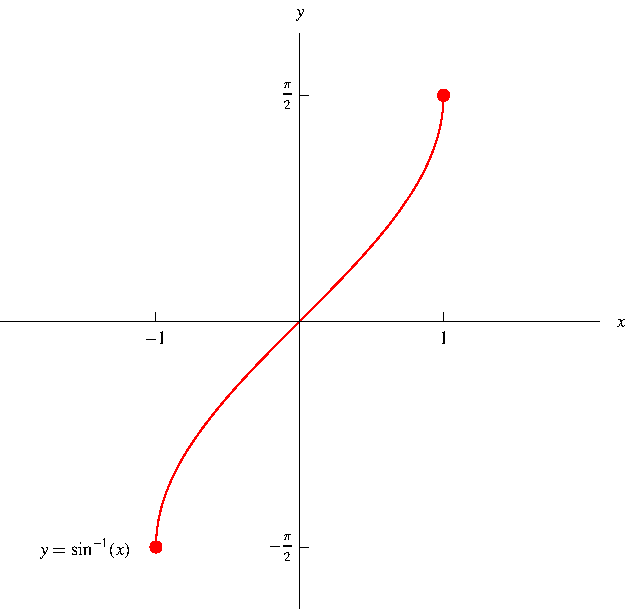
\includegraphics[height=4cm]{inverse-trig/pictures/07-06-arcsine.pdf}%
%}%

\end{columns}
\end{frame}
% end module arcsin-def

% begin module arcsin-ex1
\begin{frame}
\vskip -0.1cm
\begin{example}
\begin{columns}[t]
\column{.3\textwidth}
\hfil \hfil Find $\displaystyle \Arcsin \left( \frac{1}{2}\right)$.
\begin{itemize}
\item<2->  $\displaystyle \sin \left(\uncover<2-| handout:0>{\frac{\pi}{ 6}}\right) = \frac{1}{2}$.
\item<3->  $\displaystyle -\frac{\pi}{2} \leq \uncover<3-| handout:0>{\frac{\pi}{6}} \leq \frac{\pi}{2}$.
\item<4->  Therefore $ \Arcsin \left( \frac{1}{2}\right) = \uncover<3-| handout:0>{\frac{\pi}{6}}$.
\end{itemize}
\column{.7\textwidth}
\hfil \hfil Find $\displaystyle
\tan \left( \Arcsin \left( \frac{1}{3}\right) \right)
$.
\begin{itemize}
\item<5->  Let $\theta = \Arcsin \left(\frac{1}{3}\right)$, so $\sin \theta = \frac{ \alertNoH{6}{1}}{\alertNoH{7}{3}}$.
\item<6->  Draw a right triangle with  \alertNoH{6}{opposite side $1$} and \alertNoH{7}{hypotenuse $3$}.
\item<8-> Let the angle $\theta$ be as labeled. \uncover<9->{ Then $ \alertNoH{9,10}{\sin\theta= \frac{1 }{3}}$ \uncover<10->{and so $\alertNoH{10}{ \theta= \arcsin\left(\frac{1}{3}\right)}$}.}
\item<11->  \alertNoH{11-12}{Length of adjacent side $ =\worksheet{ \fcAnswer{12}{\sqrt{3^2-1^2}} \uncover<13->{ = \sqrt{8} = 2\sqrt{2}.}}$}
\item<14->  Then \alertNoH{ 14-15}{$\tan \left(\Arcsin \left(\frac{1}{3}\right)\right) = \fcAnswer{15}{ \frac{1}{ 2\sqrt{2}}.}$}
\end{itemize}

\vskip -0.1cm
\hfil\hfil \psset{xunit=1.5cm, yunit=1.5cm}
\begin{pspicture}(-0.2, -0.35)(3.2,1.05)
\small%
\fcBoundingBox{-0.2}{-0.35}{ 10 sqrt 0.3 add}{1.15}
\psline[linecolor=red!1](2.828427125, 1)(2.828427125, 1.01)
\psline[linecolor=red!1](0, -0.35)(0.001, -0.35)
\psdot[linecolor=white](3.1, 1.0)
\psdot[linecolor=white](-0.1, -0.3)
\uncover<6->{%
\psline(0,0)(! 10 sqrt 0)(! 10 sqrt  1)(0,0)
\psline(! 10 sqrt 0.1)(! 10 sqrt 0.1)(! 10 sqrt 0)
\rput[b](1.41, 0.55){$3$}
\rput[l](! 10 sqrt 0.05 add 0.5){$1$}
\rput(0.8, 0.13){$ \alertNoH{8}{\theta}$}
\fcAngle{0}{0.339837}{0.4}{}
}
\uncover<handout:0|6,9,15>{\psline[linewidth=2pt, linecolor=blue](! 10 sqrt 0)(! 10 sqrt  1)}%
\uncover<handout:0|15>{\psline[linewidth=2pt, linecolor=green](0,0)(! 10 sqrt 0)}%
\uncover<handout:0|7,9>{\psline[linewidth=2pt, linecolor=orange](! 0 0)(! 10 sqrt  1)}%
\uncover<11-| handout:0>{\rput[t](! 10 sqrt 2 div -0.1){$ \fcAnswerUncover{11}{13}{ 2 \sqrt{2}}$}}
\end{pspicture}
\end{columns}

\end{example}
\end{frame}
% end module arcsin-ex1

% begin module arcsin-derivative
\begin{frame}
\begin{theorem}[The Derivative of $\Arcsin x$]
\[
\frac{\diff}{\diff x} \left( \Arcsin x\right) = \frac{1}{\sqrt{1-x^2}}, \qquad -1 < x < 1.
\]
\end{theorem}
\begin{proof}
\abovedisplayskip=0pt
\belowdisplayskip=-15pt
\abovedisplayshortskip=0pt
\belowdisplayshortskip=0pt
\begin{align*}
\uncover<2->{%
\text{Let}\quad y %
}%
& \uncover<2->{%
 = \Arcsin x.
}\\%
\uncover<2->{%
\text{Then}\quad \alert<handout:0| 3-4,10>{\sin y} %
}%
& \uncover<2->{%
 \alert<handout:0| 10>{=}  \alert<handout:0| 5-6,10>{x}\quad \text{and} \quad \alert<handout:0| 9>{-\pi/2 \leq y \leq \pi/2}.
}\\%
\uncover<3->{%
\text{Differentiate implicitly:}\quad \alert<handout:0| 3-4>{\uncover<4->{\cos y \cdot y'}} %
}%
& \uncover<3->{%
 = \uncover<6->{\alert<handout:0| 6>{1}} 
}\\%
\uncover<7->{%
y' %
}%
& \uncover<7->{%
 = \frac{1}{\alert<handout:0| 8>{\cos y}} %
}\\%
& \uncover<8->{%
 = \frac{1}{\alert<handout:0| 8>{\alert<handout:0| 9>{\pm}\sqrt{1-\sin^2y}}} %
}\\%
\uncover<9->{%
\text{But \alert<handout:0| 9>{$\cos y > 0$}:}\quad %
}%
& \uncover<9->{%
 = \frac{1}{\sqrt{1-\alert<handout:0| 10>{\sin^2y}}} %
}%
\uncover<10->{%
 = \frac{1}{\sqrt{1-\alert<handout:0| 10>{x^2}}}. \qedhere%
}%
\end{align*}
\end{proof}
\end{frame}
% end module arcsin-derivative

% begin module arcsin-properties
\begin{frame}
Important facts about $\Arcsin$:
\begin{columns}[c]
\column{.5\textwidth}
\psset{xunit=2cm,yunit=2cm}
\begin{pspicture}(-1.5,-2)(1.6,2.1)
\tiny
\psaxes[ticks=none, labels=none]{<->}(0,0)(-1.5,-2)(1.5,2)
\fcLabels{1.5}{2}
\fcLabelXOne
\psline(-1, -0.1)(-1,0.1)
\rput[t](-1,  -0.1){$-1$}

\psline(-0.1, 1.570796327)(0.1,1.570796327)
\rput[r](-0.1,  1.570796327){$\frac{\pi}{2}$}
\psline(-0.1, -1.570796327)(0.1,-1.570796327)
\rput[r](-0.1,  -1.570796327){$-\frac{\pi}{2}$}

\psplot[linecolor=red, plotpoints=1000]{-1}{1}{x ASIN}
\rput[rb](-0.05, 0.2){$y=\Arcsin x$}
\fcFullDot{1}{1.570796327}
\fcFullDot{-1}{-1.570796327}
\uncover<3| handout:0>{\psline[linecolor=red, linewidth=2pt]{<->}(-1,0)(1,0) }
\uncover<5| handout:0>{\psline[linecolor=red, linewidth=2pt]{<->}(0,-1.570796327)(0,1.570796327) }

\end{pspicture}
\column{.5\textwidth}
\begin{enumerate}
\item  \alert<handout:0| 2-3>{Domain: \uncover<3-| handout:0>{$[-1, 1]$.}}
\item  \alert<handout:0| 4-5>{Range: \uncover<5-| handout:0>{$[-\pi /2, \pi /2]$.}}
\item  $\Arcsin x = y \Leftrightarrow \sin y = x$ and $-\pi /2 \leq y \leq \pi /2$.
\item  $\Arcsin (\sin x) = x$ for $-\pi /2 \leq x \leq \pi /2$.
\item  $\sin (\Arcsin x) = x$ for $-1 \leq x \leq 1$.
\item  $\frac{\diff}{\diff x} (\Arcsin x) = \frac{1}{\sqrt{1-x^2}}$.
\end{enumerate}
\end{columns}
\end{frame}
% end module arcsin-properties


% begin module arccos-def
\begin{frame}
%\ \only<handout:0| -1>{%
%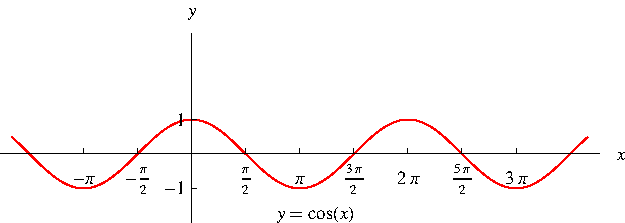
\includegraphics[width=12cm]{inverse-trig/pictures/07-06-arccosa.pdf}%
%}%
%\only<2>{%
%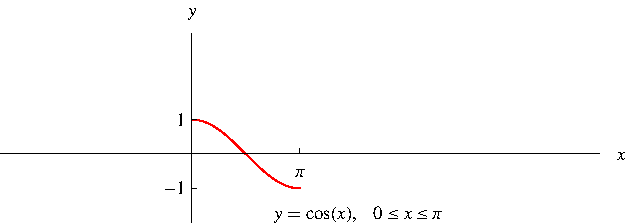
\includegraphics[width=12cm]{inverse-trig/pictures/07-06-arccosb.pdf}%
%}%
%\only<handout:0| 3->{%
%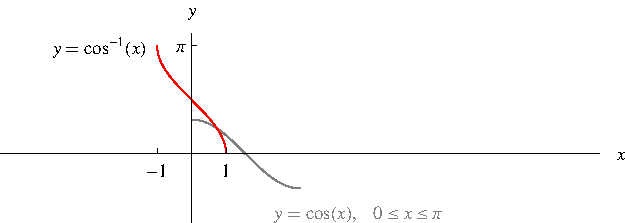
\includegraphics[width=12cm]{inverse-trig/pictures/07-06-arccosc.pdf}%
%}%
\psset{xunit=0.6cm,yunit=0.6cm}
\begin{pspicture}(-5,-1.4)(10,1.4)
\tiny
\psaxes[labels=none, ticks=x, Dx=1.570796327, Dy=1] {<->}(0,0)(-4,-1.4)(10,3.4)
\psLabels{10}{3.4}
\uncover<1>{\psplot[linecolor=red, plotpoints=1000]{-4}{10}{x 57.295779513 mul cos}
\rput[t](3.5, 1){$y=\cos x$}
}
\uncover<2>{\psplot[linecolor=red, plotpoints=1000]{0}{3.141592654}{x 57.295779513 mul cos}
\rput[t](3.5, 1){$y=\cos x, \quad 0\leq x\leq \pi$}
}
\uncover<3->{\psplot[linecolor=gray, plotpoints=1000]{0}{3.141592654}{x 57.295779513 mul cos}
\rput[t](3.5, 1){\color{gray}$y=\cos x, \quad 0\leq x\leq \pi$}

\psplot[linecolor=red, plotpoints=1000]{-1}{1}{x ACOS}
\psline(-0.1,3.141592654)(0.1,3.141592654)
\rput[l](0.15,3.141592654){$\pi$}
\psline(-1,-0.1)(-1,0.1)
\rput[t](-1,-0.1){$-1$}
\psline(1,-0.1)(1,0.1)
\rput[t](1,-0.1){$1$}
\rput[r](-0.6, 0.4){$y=\Arccos x$}
}

\rput[t](-3.14, -0.3){$-\pi$}
\rput[t](-1.57, -0.3){$-\frac{\pi}{2}$}
\rput[t](1.57, -0.3){$\frac{\pi}{2}$}
\rput[t](3.14, -0.3){$\pi$}
\rput[t](4.71, -0.3){$\frac{3\pi}{2}$}
\rput[t](6.28, -0.3){$2\pi$}
\rput[t](7.85, -0.3){$\frac{5\pi}{2}$}
\rput[t](9.42, -0.3){$3\pi$}
\rput[br](-0.2,1){\tiny $1$}

\end{pspicture}

\begin{columns}[c]
\column{.65\textwidth}
\begin{itemize}
\item<1->  Same for $\cos x$.
\item<2->  Restrict the domain to $[0, \pi ]$.
\item<3->  The inverse is called $\arccos$ or $\cos^{-1}$.
\item<5->  $\Arccos (x) = y \Leftrightarrow \cos y = x$ and $0 \leq y \leq \pi$.
\end{itemize}
\column{.35\textwidth}
\uncover<4->{%
%\uncover<4->{%
%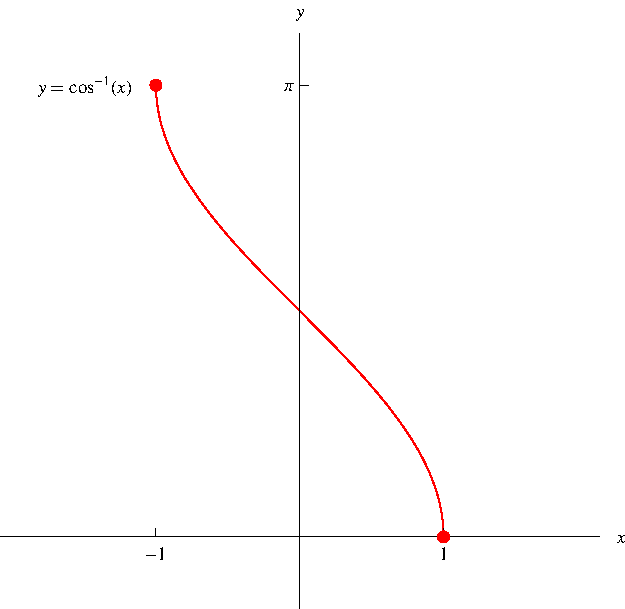
\includegraphics[height=4cm]{inverse-trig/pictures/07-06-arccosd.pdf}%
%}%
\psset{xunit=1.2cm,yunit=1.2cm}
\begin{pspicture}(-5,-1.4)(10,1.4)
\tiny
\psaxes[labels=none, ticks=none] {<->}(0,0)(-2,-0.5)(1.6,3.7)
\psLabels{1.6}{3.7}
\psplot[linecolor=red, plotpoints=1000]{-1}{1}{x ACOS}
\psline(-0.1,3.141592654)(0.1,3.141592654)
\rput[l](0.15,3.141592654){$\pi$}
\psline(-1,-0.1)(-1,0.1)
\rput[t](-1,-0.1){$-1$}
\psline(1,-0.1)(1,0.1)
\rput[t](1,-0.1){$1$}
\rput[r](-0.6, 2){$y=\Arccos x$}
\end{pspicture}
}%
\end{columns}
\end{frame}
% end module arccos-def


% begin module arccos-properties
\begin{frame}
Important facts about $\cos^{-1}$:
\begin{columns}[c]
\column{.5\textwidth}
\ 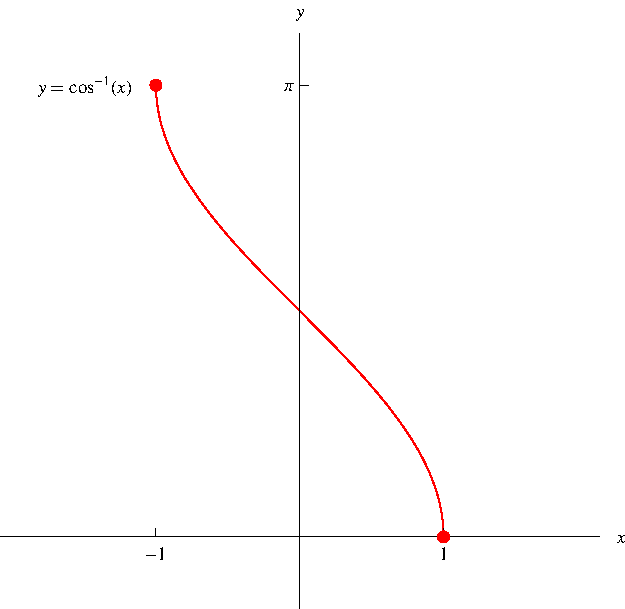
\includegraphics[height=6cm]{inverse-trig/pictures/07-06-arccosd.pdf}%
\column{.5\textwidth}
\begin{enumerate}
\item  \alert<handout:0| 2-3>{Domain: \uncover<3->{$[-1, 1]$.}}
\item  \alert<handout:0| 4-5>{Range: \uncover<5->{$[0, \pi ]$.}}
\item  $\cos^{-1} x = y \Leftrightarrow \cos y = x$ and $0 \leq y \leq \pi$.
\item  $\cos^{-1} (\cos x) = x$ for $0 \leq x \leq \pi$.
\item  $\cos (\cos^{-1} x) = x$ for $-1 \leq x \leq 1$.
\item  $\frac{\diff}{\diff x} (\cos^{-1} x) = -\frac{1}{\sqrt{1-x^2}}$.  \uncover<6->{(The proof is similar to the proof of the formula for the derivative of $\sin^{-1} x$.)}
\end{enumerate}
\end{columns}
\end{frame}
% end module arccos-properties

% begin module arctan-def
\begin{frame}
\begin{columns}[c]
\column{.5\textwidth}
\ \only<handout:0| -1>{%
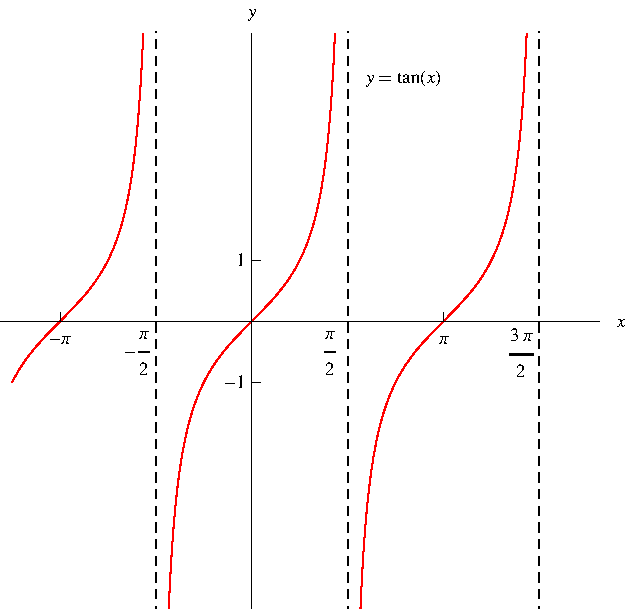
\includegraphics[width=5cm]{inverse-trig/pictures/07-06-arctana.pdf}%
}%
\only<handout:1| 2>{%
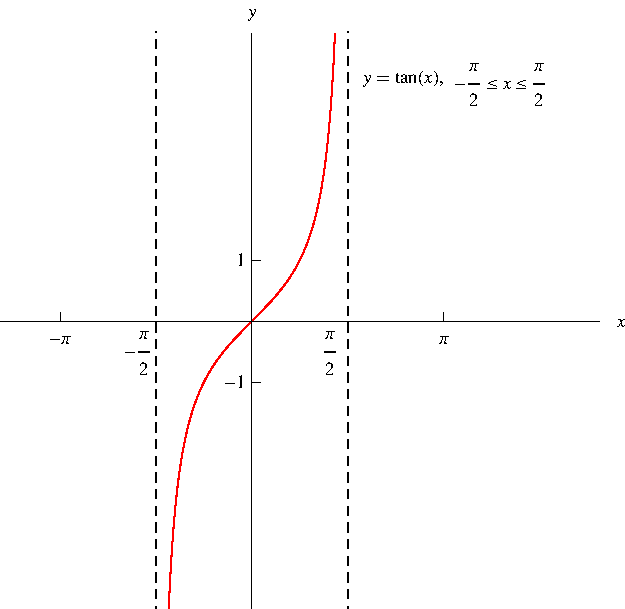
\includegraphics[width=5cm]{inverse-trig/pictures/07-06-arctanb.pdf}%
}%
\only<handout:2| 3->{%
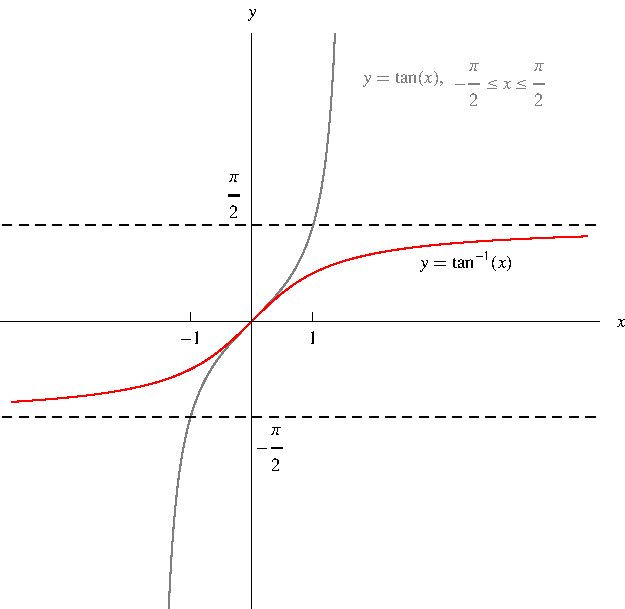
\includegraphics[width=5cm]{inverse-trig/pictures/07-06-arctanc.pdf}%
}%
\column{.5\textwidth}
\begin{itemize}
\item<1->  $\tan x$ isn't one-to-one.
\item<2->  Restrict the domain to $(-\pi /2, \pi /2)$.
\item<3->  The inverse is called $\Arctan$ or $\arctan$.
\item<4->  $\Arctan x = y \Leftrightarrow \tan y = x$ and $-\pi /2 < y < \pi /2$.
\item<5->  \alert<handout:0| 5-6>{Domain of $\Arctan$: \uncover<6-| handout:0>{$(-\infty,\infty)$.}}
\item<5->  \alert<handout:0| 7-8>{Range of $\Arctan$: \uncover<8-| handout:0>{$(-\pi / 2, \pi / 2)$.}}
\item<9->  \alert<handout:0| 9-10>{$\displaystyle \lim_{x\rightarrow \infty} \Arctan x = \uncover<10-| handout:0>{\pi / 2.}$}
\item<9->  \alert<handout:0| 11-12>{$\displaystyle \lim_{x\rightarrow - \infty} \Arctan x = \uncover<12-| handout:0>{- \pi / 2.}$}
\end{itemize}
\end{columns}
\end{frame}
% end module arctan-def

% begin module arctan-ex3
\begin{frame}
\begin{example}
Simplify the expression $\cos (\Arctan x)$.
\begin{itemize}
\item<2->  Let $y = \Arctan x$, so $\tan y = x$.
\item<3->  Draw a right triangle with opposite $x$ and adjacent $1$.
\item<4->  \alert<handout:0| 4-5>{Length of hypotenuse $ = \uncover<5->{\sqrt{1^2+x^2}.}$}
\item<6->  Then \alert<handout:0| 6-7>{$\cos (\Arctan x) = \uncover<7-| handout:0>{\frac{1}{\sqrt{1+x^2}}.}$}
\end{itemize}
\begin{pspicture}(-0.2,-0.5)(4.5,3.2)
\psframe*[linecolor=white](-0.2,-0.5)(4.5,3.2)
\psline[linecolor=red!1](4.5,-0.5)(4.5,-0.49)
\psline(0,0)(4,0)(4,3)(0,0)
\psline(3.8,0)(3.8,0.2)(4,0.2)
\fcAngle{0}{0.643501}{0.5}{$y$}
\uncover<3->{%
\rput[l](4.1, 1.5){$x$}
\rput[t](2,-0.1 ){\alertNoH{6,7}{$1$}}
}%
\uncover<5->{%
\rput[rb](1.9,1.6){\alertNoH{6,7}{$\sqrt{x^2+1}$}}
}%
\end{pspicture}
%\ \only<handout:0| -2>{%
%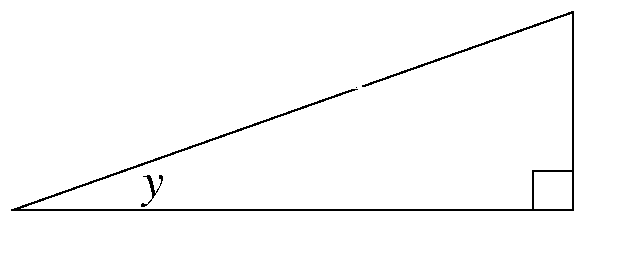
\includegraphics[width=5cm]{inverse-trig/pictures/07-06-ex3a.pdf}%
%}%
%\only<handout:0| 3-4>{%
%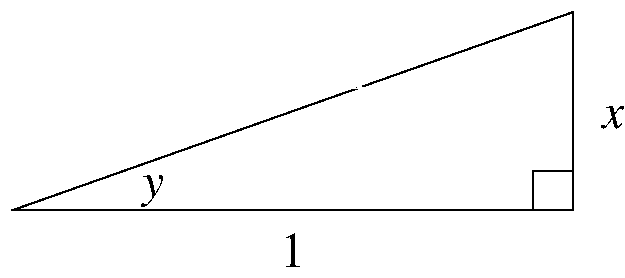
\includegraphics[width=5cm]{inverse-trig/pictures/07-06-ex3b.pdf}%
%}%
%\only<5->{%
%\includegraphics[width=5cm]{inverse-trig/pictures/07-06-ex3c.pdf}%
%}%
\end{example}
\end{frame}
% end module arctan-ex3

% begin module arctan-ex4
\begin{frame}
\begin{example}
Evaluate
\[
\lim_{x\rightarrow 2^+} \Arctan \left( \frac{1}{x-2}\right) .
\]
\uncover<2->{
\[
\frac{1}{x-2} \rightarrow \infty \qquad \text{ as } \qquad x\rightarrow 2^+.
\]
}
\uncover<3->{
Therefore
\[
\alertNoH{ 3-4}{\lim_{x\rightarrow 2^+} \Arctan \left( \frac{1}{x-2}\right) = \fcAnswer{4}{\worksheet{\frac{\pi}{2}}.}}
\]
}
\end{example}
\end{frame}
% end module arctan-ex4

% begin module arctan-derivative
\begin{frame}
\begin{theorem}[The Derivative of $\Arctan x$]
\[
\frac{\diff}{\diff x} (\Arctan x) = \frac{1}{1 + x^2}.
\]
\end{theorem}
\begin{proof}
\abovedisplayskip=0pt
\belowdisplayskip=-15pt
\abovedisplayshortskip=0pt
\belowdisplayshortskip=0pt
\begin{align*}
\uncover<2->{%
\text{Let}\quad y %
}%
& \uncover<2->{%
 = \Arctan x.
}\\%
\uncover<2->{%
\text{Then}\quad \alert<handout:0| 3-4,10>{\tan y} %
}%
& \uncover<2->{%
 \alert<handout:0| 10>{=}  \alert<handout:0| 5-6,10>{x.} %
}\\%
\uncover<3->{%
\text{Differentiate implicitly:}\quad \alert<handout:0| 3-4>{\uncover<4->{\sec^2 y \cdot y'}} %
}%
& \uncover<3->{%
 = \uncover<6->{\alert<handout:0| 6>{1}} 
}\\%
\uncover<7->{%
y' %
}%
& \uncover<7->{%
 = \frac{1}{\alert<handout:0| 8-9>{\sec^2 y}} %
}\\%
& \uncover<8->{%
 = \frac{1}{\alert<handout:0| 8-9>{\uncover<9->{1+\alert<handout:0| 10>{\tan^2 y}}}} %
}\\%
& \uncover<10->{%
 = \frac{1}{1+\alert<handout:0| 10>{x^2}}. \qedhere%
}%
\end{align*}
\end{proof}
\end{frame}
% end module arctan-derivative

% begin module inverse-trig-summary
\begin{frame}
The remaining inverse trigonometric functions aren't used often, and are summarized here.
\[
\begin{array}{llcrcl}
y = \csc^{-1} x &%
(|x| \geq 1) &%
\Leftrightarrow &%
\csc y = x &%
\text{ and } &%
y\in (0,\pi /2] \cup (\pi , 3\pi /2] \\%
y = \sec^{-1} x &%
(|x| \geq 1) &%
\Leftrightarrow &%
\sec y = x &%
\text{ and } &%
\alert<2>{y\in [0,\pi /2) \cup [\pi , 3\pi /2)} \\%
y = \cot^{-1} x &%
(|x| \in \mathbb{R}) &%
\Leftrightarrow &%
\cot y = x &%
\text{ and } &%
y\in (0,\pi )
\end{array}
\]

\ \only<handout:0| -1>{%
\includegraphics[width=5cm]{inverse-trig/pictures/07-06-seca.pdf}%
}%
\only<2->{%
\includegraphics[width=5cm]{inverse-trig/pictures/07-06-secb.pdf}%
}%
\end{frame}

\begin{frame}
Table of derivatives of inverse trigonometric functions: 
\begin{align*}
\frac{\diff}{\diff x} (\arcsin x) & = %
\frac{1}{\sqrt{1-x^2}} &%
\frac{\diff}{\diff x} (\csc^{-1} x) & = %
-\frac{1}{x\sqrt{x^2-1}} \\%
\frac{\diff}{\diff x} (\arccos x) & = %
-\frac{1}{\sqrt{1-x^2}} &%
\frac{\diff}{\diff x} (\sec^{-1} x) & = %
\frac{1}{x\sqrt{x^2-1}} \\%
\frac{\diff}{\diff x} (\arctan x) & = %
\frac{1}{1+x^2} &%
\frac{\diff}{\diff x} (\cot^{-1} x) & = %
-\frac{1}{1+x^2} %
\end{align*}
\end{frame}
% end module inverse-trig-summary

% begin module arcsin-ex5
\begin{frame}
\chainruley{\frac{1}{\sin^{-1}x}}{\sin^{-1} x}{u^{-1}}{-UU^{-2}}{\frac{1}{\sqrt{1-x^2}}}{-\frac{1}{(UU)^2\sqrt{1-x^2}}}{0}
\end{frame}
% end module arcsin-ex5

% end lecture

% begin lecture
\lect{March 21, 2014}{Lecture 16}{16}
% end lecture

% begin lecture
\lect{March 28, 2014}{Lecture 18}{18}
% end lecture

\end{document}
